\chapter{Polynomial-time reductions}\label{reductionchap}

\begin{objectives} \label[objectives]{Introduce-the-notion-of-p}

\begin{itemize}
\tightlist
\item
  Introduce the notion of \emph{polynomial-time reductions} as a way to
  relate the complexity of problems to one another.\\
\item
  See several examples of such reductions.\\
\item
  3SAT as a basic starting point for reductions.
\end{itemize}

\end{objectives}

Consider some of the problems we have encountered in
\cref{chapefficient}:

\begin{enumerate}
\def\labelenumi{\arabic{enumi}.}
\item
  The \emph{3SAT} problem: deciding whether a given 3CNF formula has a
  satisfying assignment.
\item
  Finding the \emph{longest path} in a graph.
\item
  Finding the \emph{maximum cut} in a graph.
\item
  Solving \emph{quadratic equations} over \(n\) variables
  \(x_0,\ldots,x_{n-1} \in \R\).
\end{enumerate}

All of these problems have the following properties:

\begin{itemize}
\item
  These are important problems, and people have spent significant effort
  on trying to find better algorithms for them.
\item
  Each one of these is a \emph{search} problem, whereby we search for a
  solution that is ``good'' in some easy to define sense (e.g., a long
  path, a satisfying assignment, etc.).
\item
  Each of these problems has a trivial exponential time algorithm that
  involve enumerating all possible solutions.
\item
  At the moment, for all these problems the best known algorithm is not
  much faster than the trivial one in the worst case.
\end{itemize}

In this chapter and in \cref{cooklevinchap} we will see that, despite
their apparent differences, we can relate the computational complexity
of these and many other problems. In fact, it turns out that the problem
above are \emph{computationally equivalent}, in the sense that solving
one of them immediately implies solving the others. This phenomenon,
known as \emph{\(\mathbf{NP}\) completeness}, is one of the surprising
discoveries of theoretical computer science, and we will see that it has
far-reaching ramifications.


\begin{figure}
\centering
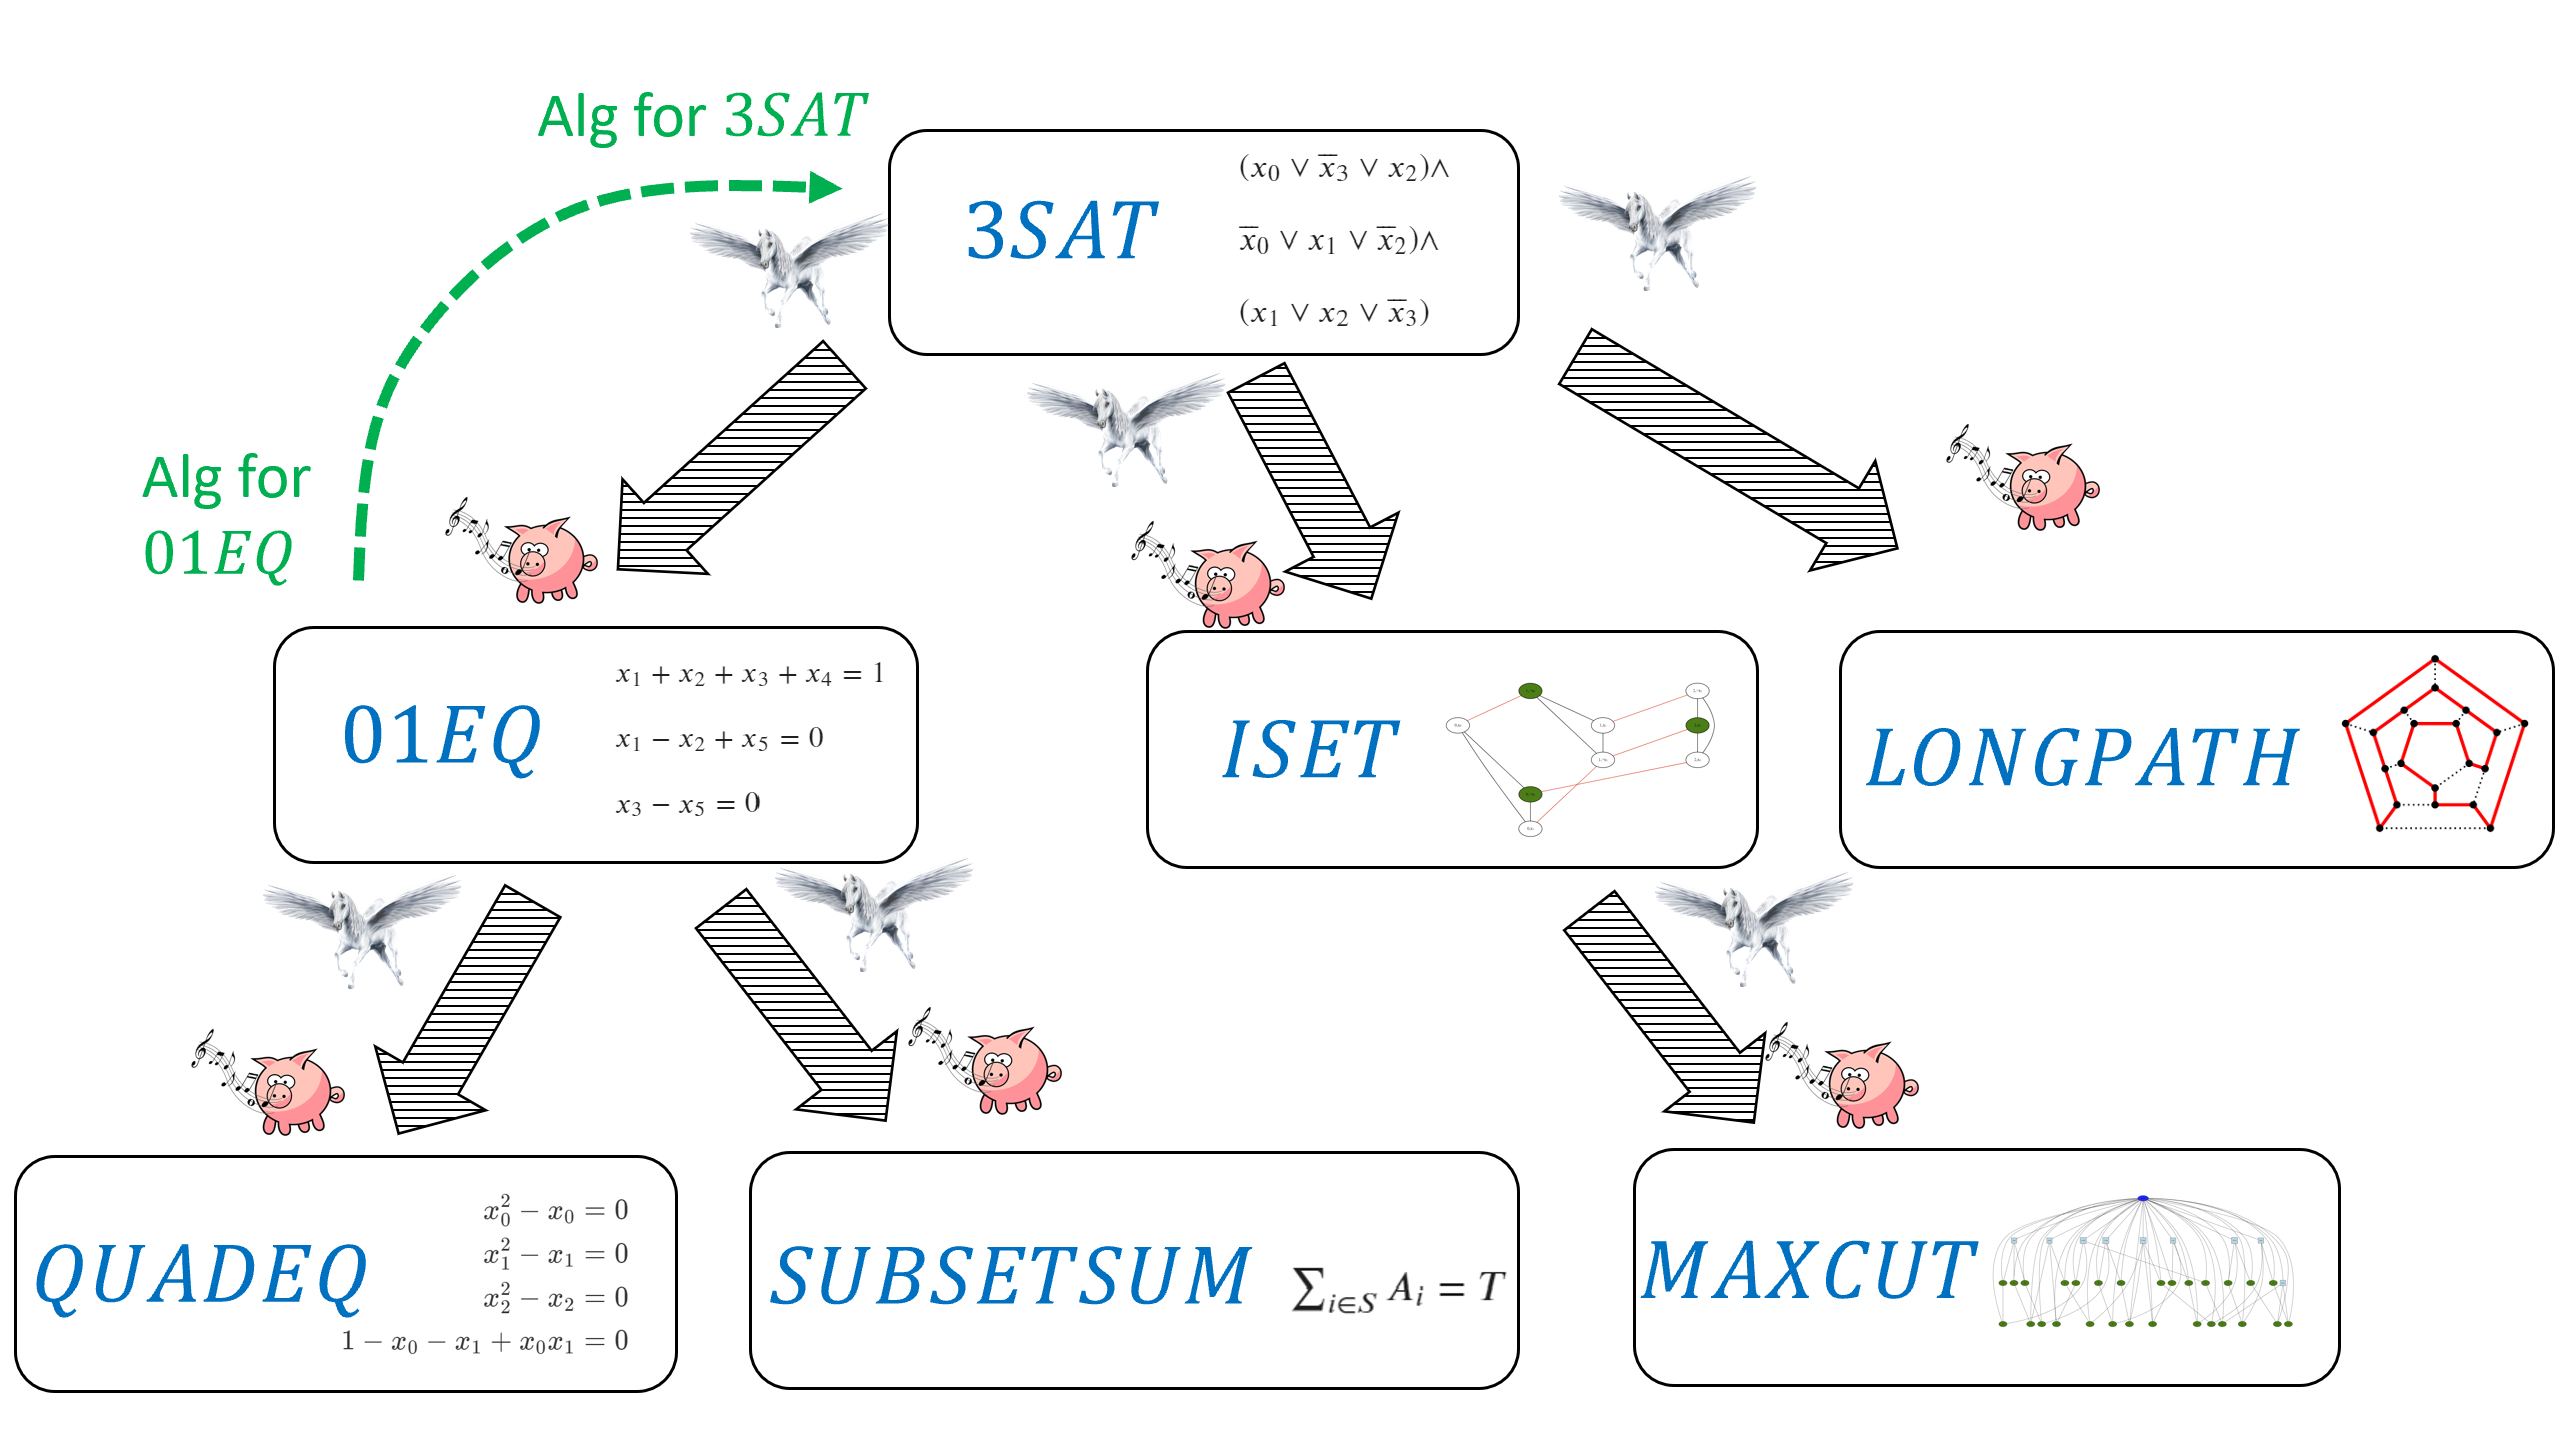
\includegraphics[width=\textwidth, height=0.25\paperheight, keepaspectratio]{../figure/reductionsoverview.png}
\caption{In this chapter we show that if the
\(3\ensuremath{\mathit{SAT}}\) problem cannot be solved in polynomial
time, then neither can the \(\ensuremath{\mathit{QUADEQ}}\),
\(\ensuremath{\mathit{LONGESTPATH}}\), \(\ensuremath{\mathit{ISET}}\)
and \(\ensuremath{\mathit{MAXCUT}}\) problems. We do this by using the
\emph{reduction paradigm} showing for example ``if pigs could whistle''
(i.e., if we had an efficient algorithm for
\(\ensuremath{\mathit{QUADEQ}}\)) then ``horses could fly'' (i.e., we
would have an efficient algorithm for \(3\ensuremath{\mathit{SAT}}\).)}
\label{reductionsoverviewfig}
\end{figure}

In this chapter we will see that for each one of the problems of finding
a longest path in a graph, solving quadratic equations, and finding the
maximum cut, if there exists a polynomial-time algorithm for this
problem then there exists a polynomial-time algorithm for the 3SAT
problem as well. In other words, we will \emph{reduce} the task of
solving 3SAT to each one of the above tasks. Another way to interpret
these results is that if there \emph{does not exist} a polynomial-time
algorithm for 3SAT then there does not exist a polynomial-time algorithm
for these other problems as well. In \cref{cooklevinchap} we will see
evidence (though no proof!) that all of the above problems do not have
polynomial-time algorithms and hence are \emph{inherently intractable}.

\section{Formal definitions of
problems}\label{formaldefdecisionexamplessec}

For reasons of technical convenience rather than anything substantial,
we concern ourselves with \emph{decision problems} (i.e., Yes/No
questions) or in other words \emph{Boolean} (i.e., one-bit output)
functions. We model the problems above as functions mapping
\(\{0,1\}^*\) to \(\{0,1\}\) in the following way:

\paragraph{3SAT.} The \emph{3SAT problem} can be phrased as the function
\(3\ensuremath{\mathit{SAT}}:\{0,1\}^* \rightarrow \{0,1\}\) that takes
as input a 3CNF formula \(\varphi\) (i.e., a formula of the form
\(C_0 \wedge \cdots \wedge C_{m-1}\) where each \(C_i\) is the OR of
three variables or their negation) and maps \(\varphi\) to \(1\) if
there exists some assignment to the variables of \(\varphi\) that causes
it to evalute to \emph{true}, and to \(0\) otherwise. For example

\[3\ensuremath{\mathit{SAT}}\left("(x_0 \vee \overline{x}_1 \vee x_2)  \wedge   (x_1 \vee x_2 \vee \overline{x_3}) \wedge (\overline{x}_0 \vee \overline{x}_2 \vee x_3)" \right)  = 1\]

since the assignment \(x = 1101\) satisfies the input formula. In the
above we assume some representation of formulas as strings, and define
the function to output \(0\) if its input is not a valid representation;
we use the same convention for all the other functions below.

\paragraph{Quadratic equations.} The \emph{quadratic equations problem}
corresponds to the function
\(\ensuremath{\mathit{QUADEQ}}:\{0,1\}^* \rightarrow \{0,1\}\) that maps
a set of quadratic equations \(E\) to \(1\) if there is an assignment
\(x\) that satisfies all equations, and to \(0\) otherwise.

\paragraph{Longest path.} The \emph{longest path problem} corresponds to
the function
\(\ensuremath{\mathit{LONGPATH}}:\{0,1\}^* \rightarrow \{0,1\}\) that
maps a graph \(G\) and a number \(k\) to \(1\) if there is a simple path
in \(G\) of length at least \(k\), and maps \((G,k)\) to \(0\)
otherwise. The longest path problem is a generalization of the
well-known
\href{https://en.wikipedia.org/wiki/Hamiltonian_path_problem}{Hamiltonian
Path Problem} of determining whether a path of length \(n\) exists in a
given \(n\) vertex graph.

\paragraph{Maximum cut.} The \emph{maximum cut problem} corresponds to
the function
\(\ensuremath{\mathit{MAXCUT}}:\{0,1\}^* \rightarrow \{0,1\}\) that maps
a graph \(G\) and a number \(k\) to \(1\) if there is a cut in \(G\)
that cuts at least \(k\) edges, and maps \((G,k)\) to \(0\) otherwise.

All of the problems above are in \(\mathbf{EXP}\) but it is not known
whether or not they are in \(\mathbf{P}\). However, we will see in this
chapter that if either \(\ensuremath{\mathit{QUADEQ}}\) ,
\(\ensuremath{\mathit{LONGPATH}}\) or \(\ensuremath{\mathit{MAXCUT}}\)
are in \(\mathbf{P}\), then so is \(3\ensuremath{\mathit{SAT}}\).

\section{Polynomial-time reductions}\label{polytimeredsec}

Suppose that \(F,G:\{0,1\}^* \rightarrow \{0,1\}\) are two functions. A
\emph{polynomial-time reduction} (or sometimes just \emph{``reduction''}
for short) from \(F\) to \(G\) is a way to show that \(F\) is ``no
harder'' than \(G\), in the sense that a polynomial-time algorithm for
\(G\) implies a polynomial-time algorithm for \(F\).

\hypertarget{reduction-def}{}
\begin{definition}[Polynomial-time reductions] \label[definition]{reduction-def}

Let \(F,G:\{0,1\}^* \rightarrow \{0,1\}^*\). We say that \emph{\(F\)
reduces to \(G\)}, denoted by \(F \leq_p G\) if there is a
polynomial-time computable \(R:\{0,1\}^* \rightarrow \{0,1\}^*\) such
that for every \(x\in \{0,1\}^*\), \[
F(x) = G(R(x)) \;. \label{eq:reduction}
\] We say that \(F\) and \(G\) have \emph{equivalent complexity} if
\(F \leq_p G\) and \(G \leq_p F\).

\end{definition}


\begin{marginfigure}
\centering
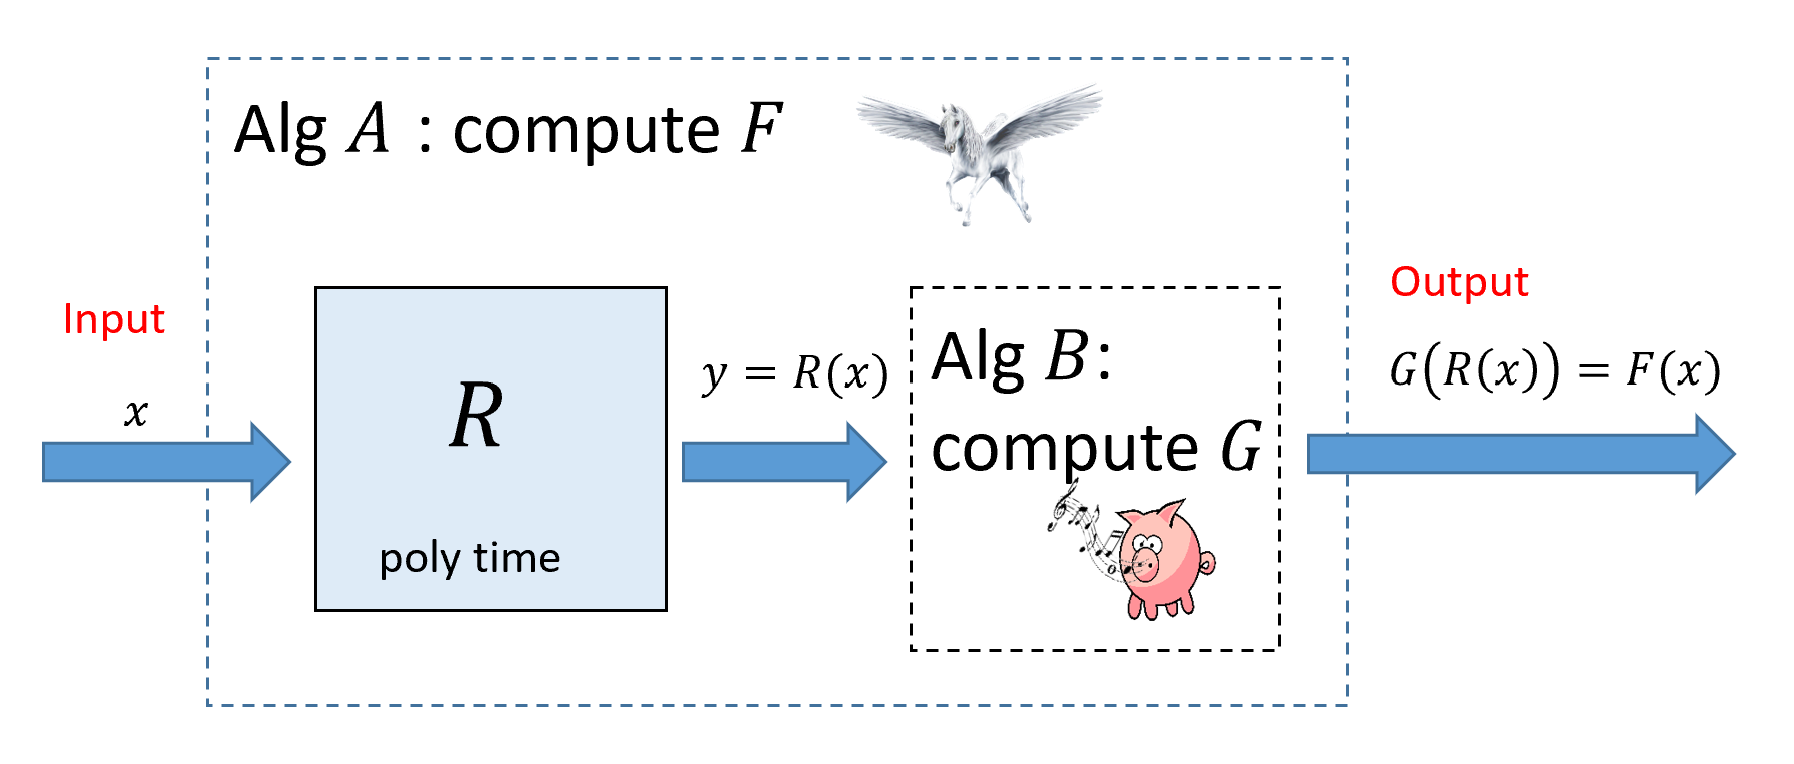
\includegraphics[width=\linewidth, height=1.5in, keepaspectratio]{../figure/reductiondescription.png}
\caption{If \(F \leq_p G\) then we can transform a polynomial-time
algorithm \(B\) that computes \(G\) into a polynomial-time algorithm
\(A\) that computes \(F\). To compute \(F(x)\) we can run the reduction
\(R\) guaranteed by the fact that \(F \leq_p G\) to obtain \(y=F(x)\)
and then run our algorithm \(B\) for \(G\) to compute \(G(y)\).}
\label{reductionsfig}
\end{marginfigure}

The following exercise justifies our intuition that \(F \leq_p G\)
signifies that "\(F\) is no harder than \(G\).

\hypertarget{reductionsandP}{}
\begin{solvedexercise}[Reductions and $\mathbf{P}$] \label[solvedexercise]{reductionsandP}

Prove that if \(F \leq_p G\) and \(G \in \mathbf{P}\) then
\(F\in \mathbf{P}\).

\end{solvedexercise}

\begin{pause} \label[pause]{As-usual-solving-this-exe}

As usual, solving this exercise on your own is an excellent way to make
sure you understand \cref{reduction-def}.

\end{pause}

\begin{solution} \label[solution]{Suppose-there-was-an-algo}

Suppose there was an algorithm \(B\) that compute \(F\) in time \(p(n)\)
where \(p\) is its input size. Then, \eqref{eq:reduction} directly gives
an algorithm \(A\) to compute \(F\) (see \cref{reductionsfig}). Indeed,
on input \(x\in \{0,1\}^*\), Algorithm \(A\) will run the
polynomial-time reduction \(R\) to obtain \(y=R(x)\) and then return
\(B(y)\). By \eqref{eq:reduction}, \(G(R(x)) = F(x)\) and hence
Algorithm \(A\) will indeed compute \(F\).

We now show that \(A\) runs in polynomial time. By assumption, \(R\) can
be computed in time \(q(n)\) for some polynomial \(q\). In particular,
this means that \(|y| \leq q(|x|)\) (as just writing down \(y\) takes
\(|y|\) steps). This, computing \(B(y)\) will take at most
\(p(|y|) \leq p(q(|x|))\) steps. Thus the total running time of \(A\) on
inputs of length \(n\) is at most the time to compute \(y\), which is
bounded by \(q(n)\), and the time to compute \(B(y)\), which is bounded
by \(p(q(n))\), and since the composition of two polynomials is a
polynomial, \(A\) runs in polynomial time.

\end{solution}

\hypertarget{reduction}{}
\begin{bigidea} \label[bigidea]{reduction}

A \emph{reduction} \(F \leq_p G\) shows that \(F\) is ``no harder than
\(G\)'' or equivalently that \(G\) is ``no easier than \(F\)''.

\end{bigidea}

A reduction from \(F\) to \(G\) can be used for two purposes:

\begin{itemize}
\item
  If we already know an algorithm for \(G\) and \(F \leq_p G\) then we
  can use the reduction to obtain an algorithm for \(F\). This is a
  widely used tool in algorithm design. For example in
  \cref{linerprogsec} we saw how the \emph{Min-Cut Max-Flow} theorem
  allows to reduce the task of computing a minimum cut in a graph to the
  task of computing a maximum flow in it.
\item
  If we have proven (or have evidence) that there exists \emph{no
  polynomial-time algorithm} for \(F\) and \(F \leq_p G\) then the
  existence of this reduction allows us to concludes that there exists
  no polynomial-time algorithm for \(G\). This is the ``if pigs could
  whistle then horses could fly'' interpretation we've seen in
  \cref{reductionsuncompsec}. We show that if there was an hypothetical
  efficient algorithm for \(G\) (a ``whistling pig'') then since
  \(F \leq_p G\) then there would be an efficient algorithm for \(F\) (a
  ``flying horse''). In this book we often use reductions for this
  second purpose, although the lines between the two is sometimes blurry
  (see the bibliographical notes in \cref{reductionsbibnotes}).
\end{itemize}

The most crucial difference between the notion in \cref{reduction-def}
and the reductions we saw in the context of \emph{uncomputability}
(e.g., in \cref{reductionsuncompsec}) is that for relating time
complexity of problems, we need the reduction to be computable in
\emph{polynomial time}, as opposed to merely computable.
\cref{reduction-def} also restricts reductions to have a very specific
format. That is, to show that \(F \leq_p G\), rather than allowing a
general algorithm for \(F\) that uses a ``magic box'' that computes
\(G\), we only allow an algorithm that computes \(F(x)\) by outputting
\(G(R(x))\). This restricted form is convenient for us, but people have
defined and used more general reductions as well (see
\cref{reductionsbibnotes}).

In this chapter we use reductions to relate the computational complexity
of the problems mentioned above: 3SAT, Quadratic Equations, Maximum Cut,
and Longest Path, as well as a few others. We will reduce 3SAT to the
latter problems, demonstrating that solving any one of them efficiently
will result in an efficient algorithm for 3SAT. In \cref{cooklevinchap}
we show the other direction: reducing each one of these problems to 3SAT
in one fell swoop.

\paragraph{Transitivity of reductions.} Since we think of \(F \leq_p G\)
as saying that (as far as polynomial-time computation is concerned)
\(F\) is ``easier or equal in difficulty to'' \(G\), we would expect
that if \(F \leq_p G\) and \(G \leq_p H\), then it would hold that
\(F \leq_p H\). Indeed this is the case:

\hypertarget{transitiveex}{}
\begin{solvedexercise}[Transitivity of polynomial-time reductions] \label[solvedexercise]{transitiveex}

For every \(F,G,H :\{0,1\}^* \rightarrow \{0,1\}\), if \(F \leq_p G\)
and \(G \leq_p H\) then \(F \leq_p H\).

\end{solvedexercise}

\begin{solution} \label[solution]{If-F-leqp-G-and-G-leqp-H-}

If \(F \leq_p G\) and \(G \leq_p H\) then there exist polynomial-time
computable functions \(R_1\) and \(R_2\) mapping \(\{0,1\}^*\) to
\(\{0,1\}^*\) such that for every \(x\in \{0,1\}^*\),
\(F(x) = G(R_1(x))\) and for every \(y\in \{0,1\}^*\),
\(G(y) = H(R_2(y))\). Combining these two equalities, we see that for
every \(x\in \{0,1\}^*\), \(F(x) = H(R_2(R_1(x)))\) and so to show that
\(F \leq_p H\), it is sufficient to show that the map
\(x \mapsto R_2(R_1(x))\) is computable in polynomial time. But if there
are some constants \(c,d\) such that \(R_1(x)\) is computable in time
\(|x|^c\) and \(R_2(y)\) is computable in time \(|y|^d\) then
\(R_2(R_1(x))\) is computable in time \((|x|^c)^d = |x|^{cd}\) which is
polynomial.

\end{solution}

\section{Reducing 3SAT to zero one
equations}\label{Reducing-SAT-to-zero-one-}

We will now show our first example of a reduction. The \emph{Zero-One
Linear Equations problem} corresponds to the function
\(01\ensuremath{\mathit{EQ}}:\{0,1\}^* \rightarrow \{0,1\}\) whose input
is a collection \(E\) of linear equations in variables
\(x_0,\ldots,x_{n-1}\), and the output is \(1\) iff there is an
assignment \(x\in \{0,1\}^n\) of \(0/1\) values to the variables that
satisfies all the equations. For example, if the input \(E\) is a string
encoding the set of equations

\[
\begin{aligned}
x_0 + x_1 + x_{2} &= 2 \\
x_0 + x_2     &= 1 \\
x_1 + x_{2} &= 2 
\end{aligned}
\]

then \(01\ensuremath{\mathit{EQ}}(E)=1\) since the assignment
\(x = 011\) satisfies all three equations. We specifically restrict
attention to linear equations in variables \(x_0,\ldots, x_{n-1}\) in
which every equation has the form \(\sum_{i \in S} x_i = b\) where
\(S \subseteq [n]\) and \(b\in \N\).\footnote{If you are familiar with
  matrix notation you may note that such equations can be written as
  \(Ax = \mathbf{b}\) where \(A\) is an \(m\times n\) matrix with
  entries in \(0/1\) and \(\mathbf{b} \in \N^m\).}

If we asked the question of whether there is a solution \(x \in \R^n\)
of \emph{real numbers} to \(E\), then this can be solved using the
famous \emph{Gaussian elimination} algorithm in polynomial time.
However, there is no known efficient algorithm to solve
\(01\ensuremath{\mathit{EQ}}\). Indeed, such an algorithm would imply an
algorithm for \(3\ensuremath{\mathit{SAT}}\) as shown by the following
theorem:

\hypertarget{tsattozoeqthm}{}
\begin{theorem}[Hardness of $01EQ$] \label[theorem]{tsattozoeqthm}

\(3\ensuremath{\mathit{SAT}} \leq_p 01\ensuremath{\mathit{EQ}}\)

\end{theorem}

\begin{proofidea} \label[proofidea]{A-constraint-x-vee-overli}

A constraint \(x_2 \vee \overline{x}_5 \vee x_7\) can be written as
\(x_2 + (1-x_5) + x_7 \geq 1\). This is a linear \emph{inequality} but
since the sum on the left-hand side is at most three, we can also turn
it into an \emph{equality} by adding two new variables \(y,z\) and
writing it as \(x_2 + (1-x_5) + x_7 + y + z =3\). (We will use fresh
such variables \(y,z\) for every constraint.) Finally, for every
variable \(x_i\) we can add a variable \(x'_i\) corresponding to its
negation by adding the equation \(x_i + x'_i = 1\), hence mapping the
original constraint \(x_2 \vee \overline{x}_5 \vee x_7\) to
\(x_2 + x'_5 + x_7 +y + z = 3\). The main \textbf{takeaway technique}
from this reduction is the idea of adding \emph{auxiliary variables} to
replace an equation such as \(x_1+x_2 +x_3 \geq 1\) that is not quite in
the form we want with the equivalent (for \(0/1\) valued variables)
equation \(x_1+x_2+x_3+u+v=3\) which is in the form we want.

\end{proofidea}


\begin{figure}
\centering
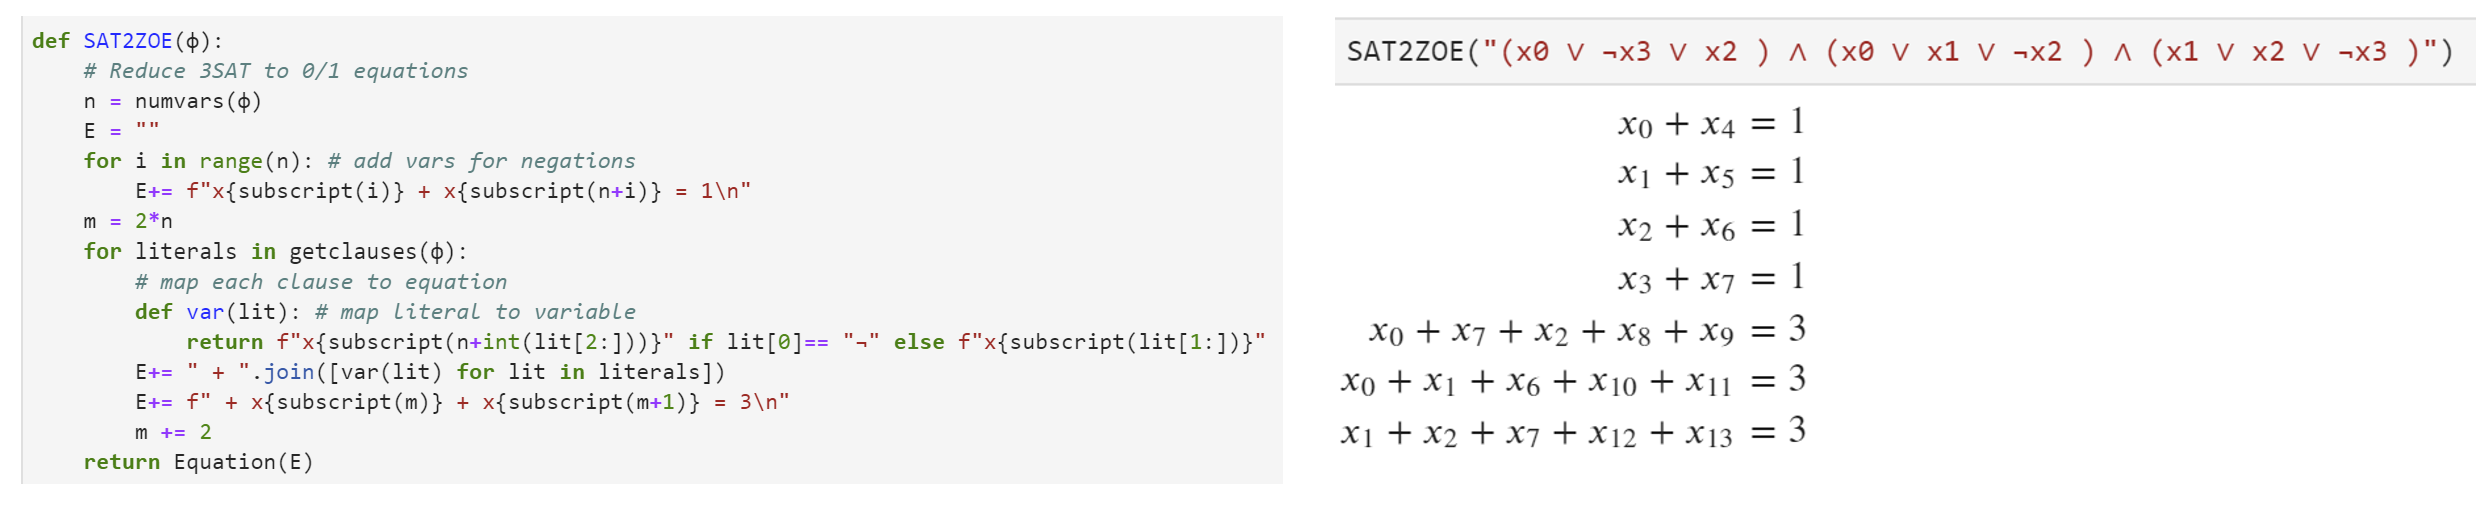
\includegraphics[width=\textwidth, height=0.25\paperheight, keepaspectratio]{../figure/3sat2zoeqreduction.png}
\caption{Left: Python code implementing the reduction of
\(3\ensuremath{\mathit{SAT}}\) to \(01\ensuremath{\mathit{EQ}}\). Right:
Example output of the reduction. Code is in our
\href{https://github.com/boazbk/tcscode}{repository}.}
\label{threesat2zoeqreductionfig}
\end{figure}

\begin{proof}[Proof of \cref{tsattozoeqthm}] \label[proof]{To-prove-the-theorem-we-n}

To prove the theorem we need to:

\begin{enumerate}
\def\labelenumi{\arabic{enumi}.}
\item
  Describe an algorithm \(R\) for mapping an input \(\varphi\) for
  \(3\ensuremath{\mathit{SAT}}\) into an input \(E\) for
  \(01\ensuremath{\mathit{EQ}}\).
\item
  Prove that the algorithm runs in polynomial time.
\item
  Prove that
  \(01\ensuremath{\mathit{EQ}}(R(\varphi)) =3\ensuremath{\mathit{SAT}}(\varphi)\)
  for every 3CNF formula \(\varphi\).
\end{enumerate}

We now proceed to do just that. Since this is our first reduction, we
will spell out this proof in detail. However it straightforwardly
follows the proof idea.

\begin{algorithm}[$3SAT$ to $01EQ$ reduction]
\label[algorithm]{zerooneeqreduction} ~ \\ \noindent
\begin{algorithmic}[1]
\INPUT  3CNF formula $\varphi$ with $n$ variables $x_0,\ldots,x_{n-1}$ and $m$ clauses.
\OUTPUT  Set $E$ of linear equations over $0/1$ such that $3SAT(\varphi)=1$ -iff $01EQ(E)=1$.
\STATE Let $E$'s variables be $x_0,\ldots,x_{n-1}$, $x'_0,\ldots,x'_{n-1}$, $y_0,\ldots,y_{m-1}$, $z_0,\ldots,z_{m-1}$.
\FOR{$i \in [n]$}
  \STATE add to $E$ the equation $x_i + x'_i = 1$
\ENDFOR
\FOR{j\in [m]}
  \STATE Let $j$-th clause be $w_1 \vee w_2 \vee w_3$ where $w_1,w_2,w_3$ are literals.
  \FOR{$a\in[3]$}
    \IF{$w_a$ is variable $x_i$}
      \STATE set $t_a \leftarrow x_i$
    \ENDIF
    \IF{$w_a$ is negation $\neg x_i$}
      \STATE set $t_a \leftarrow x'_i$
    \ENDIF
   \ENDFOR
   \STATE Add to $E$ the equation $t_1 + t_2 + t_3 + y_j + z_j = 3$.
\ENDFOR
\RETURN $E$ 
\end{algorithmic}
\end{algorithm}

The reduction is described in \cref{zerooneeqreduction}, see also
\cref{threesat2zoeqreductionfig}. If the input formula has \(n\)
variable and \(m\) steps, \cref{zerooneeqreduction} creates a set \(E\)
of \(n+m\) equations over \(2n+2m\) variables. \cref{zerooneeqreduction}
makes an initial loop of \(n\) steps (each taking constant time) and
then another loop of \(m\) steps (each taking constant time) to create
the equations, and hence it runs in polynomial time.

Let \(R\) be the function computed by \cref{zerooneeqreduction}. The
heart of the proof is to show that for every 3CNF \(\varphi\),
\(01\ensuremath{\mathit{EQ}}(R(\varphi)) = 3\ensuremath{\mathit{SAT}}(\varphi)\).
We split the proof into two parts. The first part, traditionally known
as the \textbf{completeness} property, is to show that if
\(3\ensuremath{\mathit{SAT}}(\varphi)=1\) then
\(O1\ensuremath{\mathit{EQ}}(R(\varphi))=1\). The second part,
traditionally known as the \textbf{soundness} property, is to show that
if \(01\ensuremath{\mathit{EQ}}(R(\varphi))=1\) then
\(3\ensuremath{\mathit{SAT}}(\varphi)=1\). (The names ``completeness''
and ``soundness'' derive viewing a solution to \(R(\varphi)\) as a
``proof'' that \(\varphi\) is satisfiable, in which case these
conditions corresponds to completeness and soundness as defined in
\cref{godelproofsystemssec}. However, if you find the names confusing
you can simply think of completeness as the ``\(1\)-instance maps to
\(1\)-instance'' property and soundness as the ``\(0\)-instance maps to
\(0\)-instance'' property.)

We complete the proof by showing both parts:

\begin{itemize}
\item
  \textbf{Completeness:} Suppose that
  \(3\ensuremath{\mathit{SAT}}(\varphi)=1\), which means that there is
  an assignment \(x\in \{0,1\}^n\) that satisfies \(\varphi\). We know
  that for every clause \(C_j\) in \(\varphi\) of the form
  \(w_1 \vee w_2 \vee w_3\) (with \(w_1,w_2,w_3\) being literals),
  \(w_1 + w_2 + w_3 \geq 1\), which means that we can assign values to
  \(y_j,z_j\) in \(\{0,1\}\) such that
  \(w_1 + w_2 + w_3 + y_j + z_j = 3\). This means that if we let
  \(x'_i = 1-x_i\) for every \(i\in [n]\), then the assignment
  \(x_0,\ldots,x_{n-1}\), \(x'_0,\ldots,x'_{n-1}\),
  \(y_0,\ldots,y_{m-1}\), \(z_0,\ldots,z_{m-1}\) satisfies the equations
  \(E = R(\varphi)\) and hence
  \(01\ensuremath{\mathit{EQ}}(R(\varphi))=1\).
\item
  \textbf{Soundness:} Suppose that the set of equations \(E=R(\varphi)\)
  has a satisfying assignment \(x_0,\ldots,x_{n-1}\),
  \(x'_0,\ldots,x'_{n-1}\), \(y_0,\ldots,y_{m-1}\),
  \(z_0,\ldots,z_{m-1}\). Then it must be the case that \(x'_i\) is the
  negation of \(x_i\) for all \(i\in [n]\) and since
  \(y_j + z_j \leq 2\) for every \(j\in [m]\), it must be the case that
  for every clause \(C_j\) in \(\varphi\) of the form
  \(w_1 \vee w_2 \vee w_3\) (with \(w_1,w_2,w_3\) being literals),
  \(w_1 + w_2 + w_3 \geq 1\), which means that the assignment
  \(x_0,\ldots,x_{n-1}\) satisfies \(\varphi\) and hence
  \(3\ensuremath{\mathit{SAT}}(\varphi)=1\).
\end{itemize}

\end{proof}

\paragraph{Anatomy of a reduction.} A reduction is simply an algorithm,
and like any algorithm, when we come up with a reduction, it is not
enough to describe \emph{what} the reduction does, but we also have to
provide an \emph{analysis} of \emph{why} it actually works.
Specifically, to describe a reduction \(R\) demonstrating that
\(F \leq_p G\) we need to provide the following:

\begin{itemize}
\item
  \textbf{Algorithm description:} This is the description of \emph{how}
  the algorithm maps an input into the output. For example,
  \cref{zerooneeqreduction} above is the description of how we map an
  instance of \(3\ensuremath{\mathit{SAT}}\) into an instance of
  \(01\ensuremath{\mathit{EQ}}\) in the reduction demonstrating
  \(3\ensuremath{\mathit{SAT}} \leq_p 01\ensuremath{\mathit{EQ}}\).
\item
  \textbf{Algorithm analysis:} It is not enough to describe \emph{how}
  the algorithm works but we need to also explain \emph{why} it works.
  In particular we need to provide an \emph{analysis} explaining why the
  reduction is both \emph{efficient} (i.e., runs in polynomial time) and
  \emph{correct} (satisfies that \(G(R(x)=F(x)\) for every \(x\))).
  Specifically, the components of analysis of a reduction \(R\) include:

  \begin{itemize}
  \item
    \textbf{Efficiency:} We need to show that \(R\) runs in polynomial
    time. In most reductions we encounter this part is straightforward,
    as the reductions we typically use involve a constant number of
    nested loops, each involving a constant number of operations.
  \item
    \textbf{Completeness:} In a reduction \(R\) demonstrating
    \(F \leq_p G\), the \emph{completeness} condition is the condition
    that for every \(x\in \{0,1\}^*\), if \(F(x) = 1\) then
    \(G(R(x))=1\). Typically we construct the reduction to ensure that
    this holds, by giving a way to map a ``certificate/solution''
    certifying that \(F(x)=1\) into a solution certifying that
    \(G(R(x))=1\). For example in the proof of \cref{tsattozoeqthm} the
    satisfying assignment for the \(3\ensuremath{\mathit{SAT}}\) formula
    \(\varphi\) can be mapped to a solution to the set of equations
    \(R(\varphi)\).
  \item
    \textbf{Soundness:} This is the condition that if \(F(x)=0\) then
    \(G(R(x))=0\) or (taking the contrapositive) if \(G(R(x))=1\) then
    \(F(x)=1\). This is sometimes straightforward but can also be harder
    to show than the completeness condition, and in more advanced
    reductions (such as the reduction
    \(\ensuremath{\mathit{SAT}} \leq_p \ensuremath{\mathit{ISET}}\) of
    \cref{isetnpc}) demonstrating soundness is the main part of the
    analysis.
  \end{itemize}
\end{itemize}

Whenever you need to provide a reduction, you should make sure that your
description has all these components. While it is sometimes tempting to
weave together the description of the reduction and its analysis, it is
usually clearer if you separate the two, and also break down the
analysis to its three components of efficiency, completeness, and
soundness.

\subsection{Quadratic equations}\label{Quadratic-equations}

Now that we reduced \(3\ensuremath{\mathit{SAT}}\) to
\(01\ensuremath{\mathit{EQ}}\), we can use this to reduce
\(3\ensuremath{\mathit{SAT}}\) to the \emph{quadratic equations}
problem. This is the function \(\ensuremath{\mathit{QUADEQ}}\) in which
the input is a list of \(n\)-variate polynomials
\(p_0,\ldots,p_{m-1}:\R^n \rightarrow \R\) that are all of
\href{https://en.wikipedia.org/wiki/Degree_of_a_polynomial}{degree} at
most two (i.e., they are \emph{quadratic}) and with integer
coefficients. (The latter condition is for convenience and can be
achieved by scaling.) We define
\(\ensuremath{\mathit{QUADEQ}}(p_0,\ldots,p_{m-1})\) to equal \(1\) if
and only if there is a solution \(x\in \R^n\) to the equations
\(p_0(x)=0\), \(p_1(x)=0\), \(\ldots\), \(p_{m-1}(x)=0\).

For example, the following is a set of quadratic equations over the
variables \(x_0,x_1,x_2\): \[
\begin{aligned}
x_0^2 - x_0 &= 0 \\
x_1^2 - x_1 &= 0 \\
x_2^2 - x_2 &= 0 \\
1-x_0-x_1+x_0x_1    &= 0
\end{aligned}
\] You can verify that \(x \in \R^3\) satisfies this set of equations if
and only if \(x \in \{0,1\}^3\) and \(x_0 \vee x_1 = 1\).

\hypertarget{quadeq-thm}{}
\begin{theorem}[Hardness of quadratic equations] \label[theorem]{quadeq-thm}

\[3\ensuremath{\mathit{SAT}} \leq_p \ensuremath{\mathit{QUADEQ}}\]

\end{theorem}

\begin{proofidea} \label[proofidea]{Using-the-transitivity-of}

Using the transitivity of reductions (\cref{transitiveex}), it is enough
to show that
\(01\ensuremath{\mathit{EQ}} \leq_p \ensuremath{\mathit{QUADEQ}}\), but
this follows since we can phrase the equation \(x_i \in \{0,1\}\) as the
quadratic constraint \(x_i^2 - x_i = 0\). The \textbf{takeaway
technique} of this reduction is that we can use \emph{nonlinearity} to
force continuous variables (e.g., variables taking values in \(\R\)) to
be discrete (e.g., take values in \(\{0,1\}\)).

\end{proofidea}

\begin{proof}[Proof of \cref{quadeq-thm}] \label[proof]{By-creftsattozoeqthm-and-}

By \cref{tsattozoeqthm} and \cref{transitiveex}, it is sufficient to
prove that
\(01\ensuremath{\mathit{EQ}} \leq_p \ensuremath{\mathit{QUADEQ}}\). Let
\(E\) be an instance of \(01\ensuremath{\mathit{EQ}}\) with variables
\(x_0,\ldots,x_{m-1}\). We define \(R(E)\) to be the set of quadratic
equations \(E'\) that is obtained by taking the linear equations in
\(E\) and adding to them the \(n\) quadratic equations
\(x_i^2 - x_i = 0\) for all \(i\in [n]\). Clearly the map
\(E \mapsto E'\) can be computed in polynomial time. We claim that
\(01\ensuremath{\mathit{EQ}}(E)=1\) if and only if
\(\ensuremath{\mathit{QUADEQ}}(E')=1\). Indeed, the only difference
between the two instances is that:

\begin{itemize}
\item
  In the \(01\ensuremath{\mathit{EQ}}\) instance \(E\), the equations
  are over variables \(x_0,\ldots,x_{n-1}\) in \(\{0,1\}\).
\item
  In the \(\ensuremath{\mathit{QUADEQ}}\) instance \(E'\), the equations
  are overvariables \(x_0,\ldots,x_{n-1} \in \R\) but we have the extra
  constraints \(x_i^2 - x_i = 0\) for all \(i\in [n]\).
\end{itemize}

Since for every \(a\in \R\), \(a^2 - a = 0\) if and only if
\(a \in \{0,1\}\), the two sets of equations are equivalent and
\(01\ensuremath{\mathit{EQ}}(E)=\ensuremath{\mathit{QUADEQ}}(E')\) which
is what we wanted to prove.

\end{proof}

\section{The independent set problem}\label{The-independent-set-probl}

For a graph \(G=(V,E)\), an
\href{https://en.wikipedia.org/wiki/Independent_set_(graph_theory)}{independent
set} (also known as a \emph{stable set}) is a subset \(S \subseteq V\)
such that there are no edges with both endpoints in \(S\) (in other
words, \(E(S,S)=\emptyset\)). Every ``singleton'' (set consisting of a
single vertex) is trivially an independent set, but finding larger
independent sets can be challenging. The \emph{maximum independent set}
problem (henceforth simply ``independent set'') is the task of finding
the largest independent set in the graph. The independent set problem is
naturally related to \emph{scheduling problems}: if we put an edge
between two conflicting tasks, then an independent set corresponds to a
set of tasks that can all be scheduled together without conflicts. The
independent set problem has been studied in a variety of settings,
including for example in the case of algorithms for finding structure in
\href{https://www.ncbi.nlm.nih.gov/pmc/articles/PMC3919085/}{protein-protein
interaction graphs}.

As mentioned in \cref{formaldefdecisionexamplessec}, we think of the
independent set problem as the function
\(\ensuremath{\mathit{ISET}}:\{0,1\}^* \rightarrow \{0,1\}\) that on
input a graph \(G\) and a number \(k\) outputs \(1\) if and only if the
graph \(G\) contains an independent set of size at least \(k\). We now
reduce 3SAT to Independent set.

\hypertarget{isetnpc}{}
\begin{theorem}[Hardness of Independent Set] \label[theorem]{isetnpc}

\(3\ensuremath{\mathit{SAT}} \leq_p \ensuremath{\mathit{ISET}}\).

\end{theorem}

\begin{proofidea} \label[proofidea]{The-idea-is-that-finding-}

The idea is that finding a satisfying assignment to a 3SAT formula
corresponds to satisfying many local constraints without creating any
conflicts. One can think of ``\(x_{17}=0\)'' and ``\(x_{17}=1\)'' as two
conflicting events, and of the constraints
\(x_{17} \vee \overline{x}_5 \vee x_9\) as creating a conflict between
the events ``\(x_{17}=0\)'', ``\(x_5=1\)'' and ``\(x_9=0\)'', saying
that these three cannot simultaneosly co-occur. Using these ideas, we
can we can think of solving a 3SAT problem as trying to schedule non
conflicting events, though the devil is, as usual, in the details. The
\textbf{takeaway technique} here is to map each clause of the original
formula into a \emph{gadget} which is a small subgraph (or more
generally ``subinstance'') satisfying some convenient properties. We
will see these ``gadgets'' used time and again in the construction of
polynomial-time reductions.

\end{proofidea}


\begin{marginfigure}
\centering
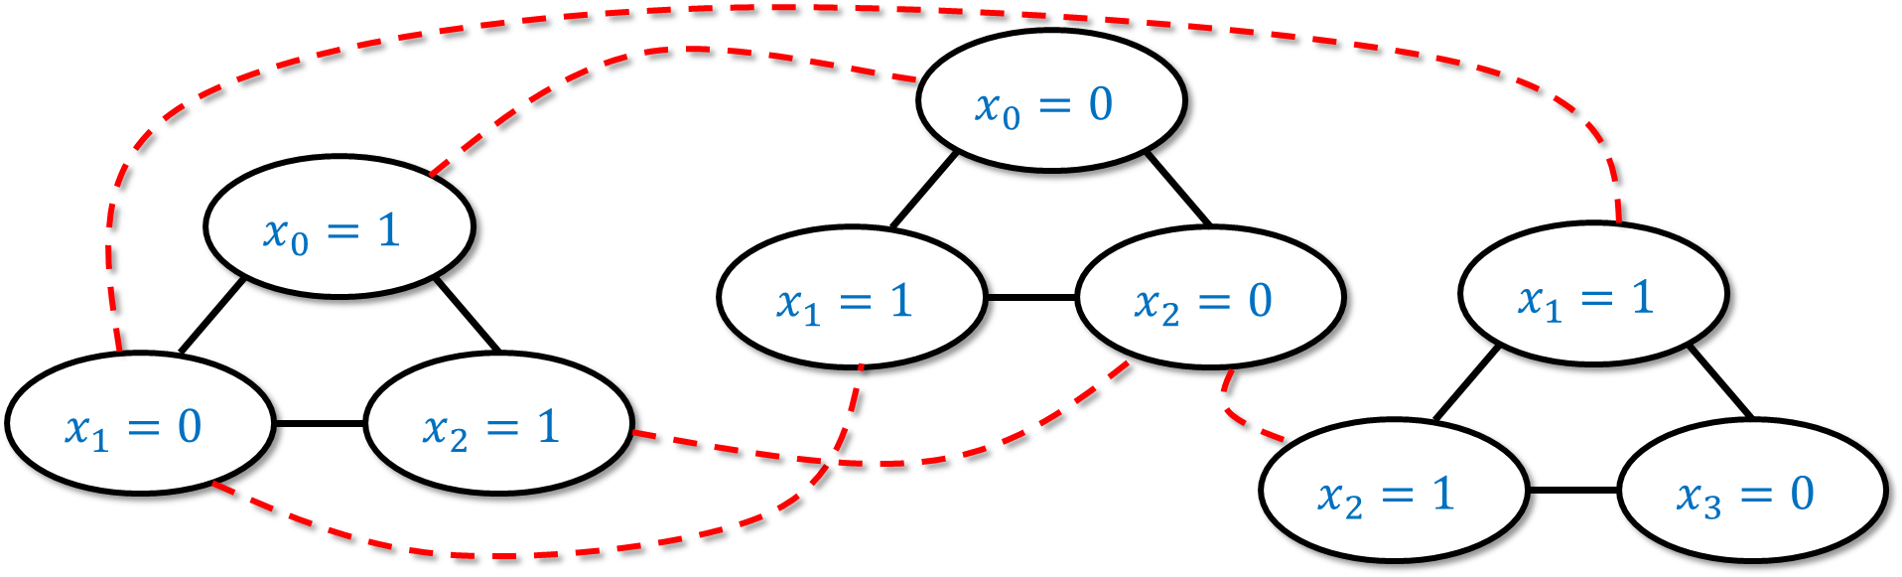
\includegraphics[width=\linewidth, height=1.5in, keepaspectratio]{../figure/example3sat2iset.png}
\caption{An example of the reduction of \(3\ensuremath{\mathit{SAT}}\)
to \(\ensuremath{\mathit{ISET}}\) for the case the original input
formula is
\(\varphi = (x_0 \vee \overline{x}_1 \vee x_2) \wedge (\overline{x}_0 \vee x_1 \vee \overline{x}_2) \wedge (x_1 \vee x_2 \vee \overline{x}_3)\).
We map each clause of \(\varphi\) to a triangle of three vertices, each
tagged above with ``\(x_i = 0\)'' or ``\(x_i=1\)'' depending on the
value of \(x_i\) that would satisfy the particular literal. We put an
edge between every two literals that are \emph{conflicting} (i.e.,
tagged with ``\(x_i=0\)'' and ``\(x_i=1\)'' respectively).}
\label{example3sat2isetfig}
\end{marginfigure}

\begin{proof}[Proof of \cref{isetnpc}] \label[proof]{Given-a-SAT-formula-varph}

Given a 3SAT formula \(\varphi\) on \(n\) variables and with \(m\)
clauses, we will create a graph \(G\) with \(3m\) vertices as follows.
(See \cref{example3sat2isetfig} for an example and
\cref{threesattoisfig} for Python code.)

\begin{itemize}
\item
  A clause \(C\) in \(\varphi\) has the form \(C = y \vee y' \vee y''\)
  where \(y,y',y''\) are \emph{literals} (variables or their negation).
  For each such clause \(C\), we will add three vertices to \(G\), and
  label them \((C,y)\), \((C,y')\), and \((C,y'')\) respectively. We
  will also add the three edges between all pairs of these vertices, so
  they form a \emph{triangle}. Since there are \(m\) clauses in
  \(\varphi\), the graph \(G\) will have \(3m\) vertices.
\item
  In addition to the above edges, we also add an edge between every pair
  vertices of the form \((C,y)\) and \((C',y')\) where \(y\) and \(y'\)
  are \emph{conflicting} literals. That is, we add an edge between
  \((C,y)\) and \((C,y')\) if there is an \(i\) such that \(y=x_i\) and
  \(y' = \overline{x}_i\) or vice versa.
\end{itemize}

The above construction of \(G\) based on \(\varphi\) can clearly be
carried out in polynomial time. Hence to prove the theorem we need to
show that \(\varphi\) is satisfiable if and only if \(G\) contains an
independent set of \(m\) vertices. We now show both directions of this
equivalence:

\textbf{Part 1: Completeness.} The ``completeness'' direction is to show
that if \(\varphi\) has a satisfying assignment \(x^*\), then \(G\) has
an independent set \(S^*\) of \(m\) vertices. Let us now show this.

Indeed, suppose that \(\varphi\) has a satisfying assignment
\(x^* \in \{0,1\}^n\). Then for every clause \(C = y \vee y' \vee y''\)
of \(\varphi\), one of the literals \(y,y',y''\) must evaluate to
\emph{true} under the assignment \(x^*\) (as otherwise it would not
satisfy \(\varphi\)). We let \(S\) be a set of \(m\) vertices that is
obtained by choosing for every clause \(C\) one vertex of the form
\((C,y)\) such that \(y\) evaluates to true under \(x^*\). (If there is
more than one such vertex for the same \(C\), we arbitrarily choose one
of them.)

We claim that \(S\) is an independent set. Indeed, suppose otherwise
that there was a pair of vertices \((C,y)\) and \((C',y')\) in \(S\)
that have an edge between them. Since we picked one vertex out of each
triangle corresponding to a clause, it must be that \(C \neq C'\). Hence
the only way that there is an edge between \((C,y)\) and \((C,y')\) is
if \(y\) and \(y'\) are conflicting literals (i.e.~\(y=x_i\) and
\(y'=\overline{x}_i\) for some \(i\)). But that would that they can't
both evaluate to \emph{true} under the assignment \(x^*\), which
contradicts the way we constructed the set \(S\). This completes the
proof of the completeness condition.

\textbf{Part 2: Soundness.} The ``soundness'' direction is to show that
if \(G\) has an independent set \(S^*\) of \(m\) vertices, then
\(\varphi\) has a satisfying assignment \(x^* \in \{0,1\}^n\). Let us
now show this.

Indeed, suppose that \(G\) has an independent set \(S*\) with \(m\)
vertices. We will define an assignment \(x^* \in \{0,1\}^n\) for the
variables of \(\varphi\) as follows. For every \(i\in [n]\), we set
\(x^*_i\) according to the following rules:

\begin{itemize}
\item
  If \(S^*\) contains a vertex of the form \((C,x_i)\) then we set
  \(x^*_i=1\).
\item
  If \(S^*\) contains a vertex of the form \((C,\overline{x_i})\) then
  we set \(x^*_i=0\).
\item
  If \(S^*\) does not contain a vertex of either of these forms, then it
  does not matter which value we give to \(x^*_i\), but for concreteness
  we'll set \(x^*_i=0\).
\end{itemize}

The first observation is that \(x^*\) is indeed well defined, in the
sense that the rules above do not conflict with one another, and ask to
set \(x^*_i\) to be both \(0\) and \(1\). This follows from the fact
that \(S^*\) is an \emph{independent set} and hence if it contains a
vertex of the form \((C,x_i)\) then it cannot contain a vertex of the
form \((C',\overline{x_i})\).

We now claim that \(x^*\) is a satisfying assignment for \(\varphi\).
Indeed, since \(S^*\) is an independent set, it cannot have more than
one vertex inside each one of the \(m\) triangles
\((C,y),(C,y'),(C,y'')\) corresponding to a clause of \(\varphi\). Hence
since \(|S^*|=m\), it must have exactly one vertex in each such
triangle. For every clause \(C\) of \(\varphi\), if \((C,y)\) is the
vertex in \(S^*\) in the triangle corresponding to \(C\), then by the
way we defined \(x^*\), the literal \(y\) must evaluate to \emph{true},
which means that \(x^*\) satisfies this clause. Therefore \(x^*\)
satisfies all clauses of \(\varphi\), which is the definition of a
satisfying assignment.

This completes the proof of \cref{isetnpc}

\end{proof}


\begin{figure}
\centering
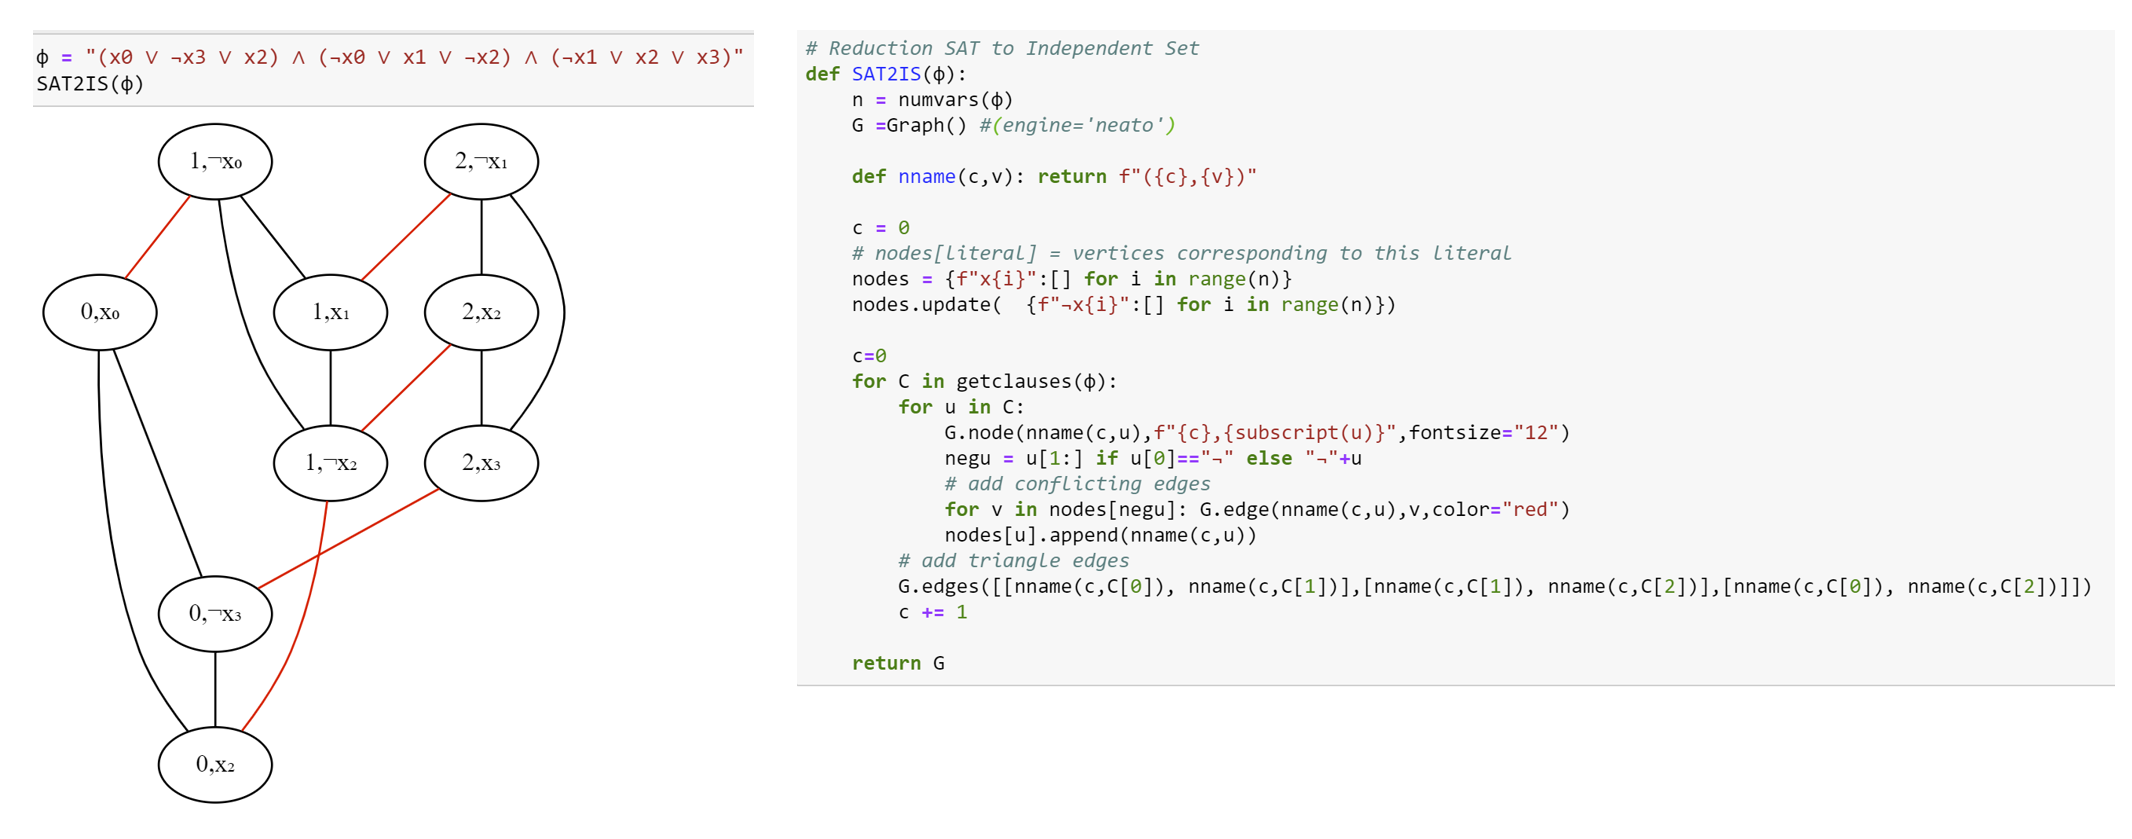
\includegraphics[width=\textwidth, height=0.25\paperheight, keepaspectratio]{../figure/3sat2ISreduction.png}
\caption{The reduction of 3SAT to Independent Set. On the righthand side
is \emph{Python} code that implements this reduction. On the lefthand
side is a sample output of the reduction. We use black for the
``triangle edges'' and red for the ``conflict edges''. Note that the
satisfying assignment \(x^* = 0110\) corresponds to the independent set
\((0,\neg x_3)\), \((1, \neg x_0)\), \((2,x_2)\).}
\label{threesattoisfig}
\end{figure}

\hypertarget{iscliqueex}{}
\begin{solvedexercise}[Clique is equivalent to independent set] \label[solvedexercise]{iscliqueex}

The \href{https://en.wikipedia.org/wiki/Clique_problem}{maximum clique
problem} corresponds to the function
\(\ensuremath{\mathit{CLIQUE}}:\{0,1\}^* \rightarrow \{0,1\}\) such that
for a graph \(G\) and a number \(k\),
\(\ensuremath{\mathit{CLIQUE}}(G,k)=1\) iff there is a \(S\) subset of
\(k\) vertices such that for \emph{every} distinct \(u,v \in S\), the
edge \(u,v\) is in \(G\). Such a set is known as a \emph{clique}.

Prove that
\(\ensuremath{\mathit{CLIQUE}} \leq_p \ensuremath{\mathit{ISET}}\) and
\(\ensuremath{\mathit{ISET}} \leq_p \ensuremath{\mathit{CLIQUE}}\).

\end{solvedexercise}

\begin{solution} \label[solution]{If-GVE-is-a-graph-we-deno}

If \(G=(V,E)\) is a graph, we denote by \(\overline{G}\) its
\emph{complement} which is the graph on the same vertices \(V\) and such
that for every distinct \(u,v \in V\), the edge \(\{u,v\}\) is present
in \(\overline{G}\) if and only if this edge is \emph{not} present in
\(G\).

This means that for every set \(S\), \(S\) is an independent set in
\(G\) if and only if \(S\) is a \emph{clique} in \(\overline{S}\).
Therefore for every \(k\),
\(\ensuremath{\mathit{ISET}}(G,k)=\ensuremath{\mathit{CLIQUE}}(\overline{G},k)\).
Since the map \(G \mapsto \overline{G}\) can be computed efficiently,
this yields a reduction
\(\ensuremath{\mathit{ISET}} \leq_p \ensuremath{\mathit{CLIQUE}}\).
Moreover, since \(\overline{\overline{G}}=G\) this yields a reduction in
the other direction as well.

\end{solution}

\section{Reducing Independent Set to Maximum
Cut}\label{Reducing-Independent-Set-}

We now show that the independent set problem reduces to the
\emph{maximum cut} (or ``max cut'') problem, modeled as the function
\(\ensuremath{\mathit{MAXCUT}}\) that on input a pair \((G,k)\) outputs
\(1\) iff \(G\) contains a cut of at least \(k\) edges. Since both are
graph problems, a reduction from independent set to max cut maps one
graph into the other, but as we will see the output graph does not have
to have the same vertices or edges as the input graph.

\hypertarget{isettomaxcut}{}
\begin{theorem}[Hardness of Max Cut] \label[theorem]{isettomaxcut}

\(\ensuremath{\mathit{ISET}} \leq_p \ensuremath{\mathit{MAXCUT}}\)

\end{theorem}

\begin{proofidea} \label[proofidea]{We-will-map-a-graph-G-int}

We will map a graph \(G\) into a graph \(H\) such that a large
independent set in \(G\) becomes a partition cutting many edges in
\(H\). We can think of a cut in \(H\) as coloring each vertex either
``blue'' or ``red''. We will add a special ``source'' vertex \(s^*\),
connect it to all other vertices, and assume without loss of generality
that it is colored blue. Hence the more vertices we color red, the more
edges from \(s^*\) we cut. Now, for every edge \(u,v\) in the original
graph \(G\) we will add a special ``gadget'' which will be a small
subgraph that involves \(u\),\(v\), the source \(s^*\), and two other
additional vertices. We design the gadget in a way so that if the red
vertices are not an independent set in \(G\) then the corresponding cut
in \(H\) will be ``penalized'' in the sense that it would not cut as
many edges. Once we set for ourselves this objective, it is not hard to
find a gadget that achieves it\(-\) see the proof below. Once again the
\textbf{takeaway technique} is to use (this time a slightly more clever)
gadget.

\end{proofidea}


\begin{figure}
\centering
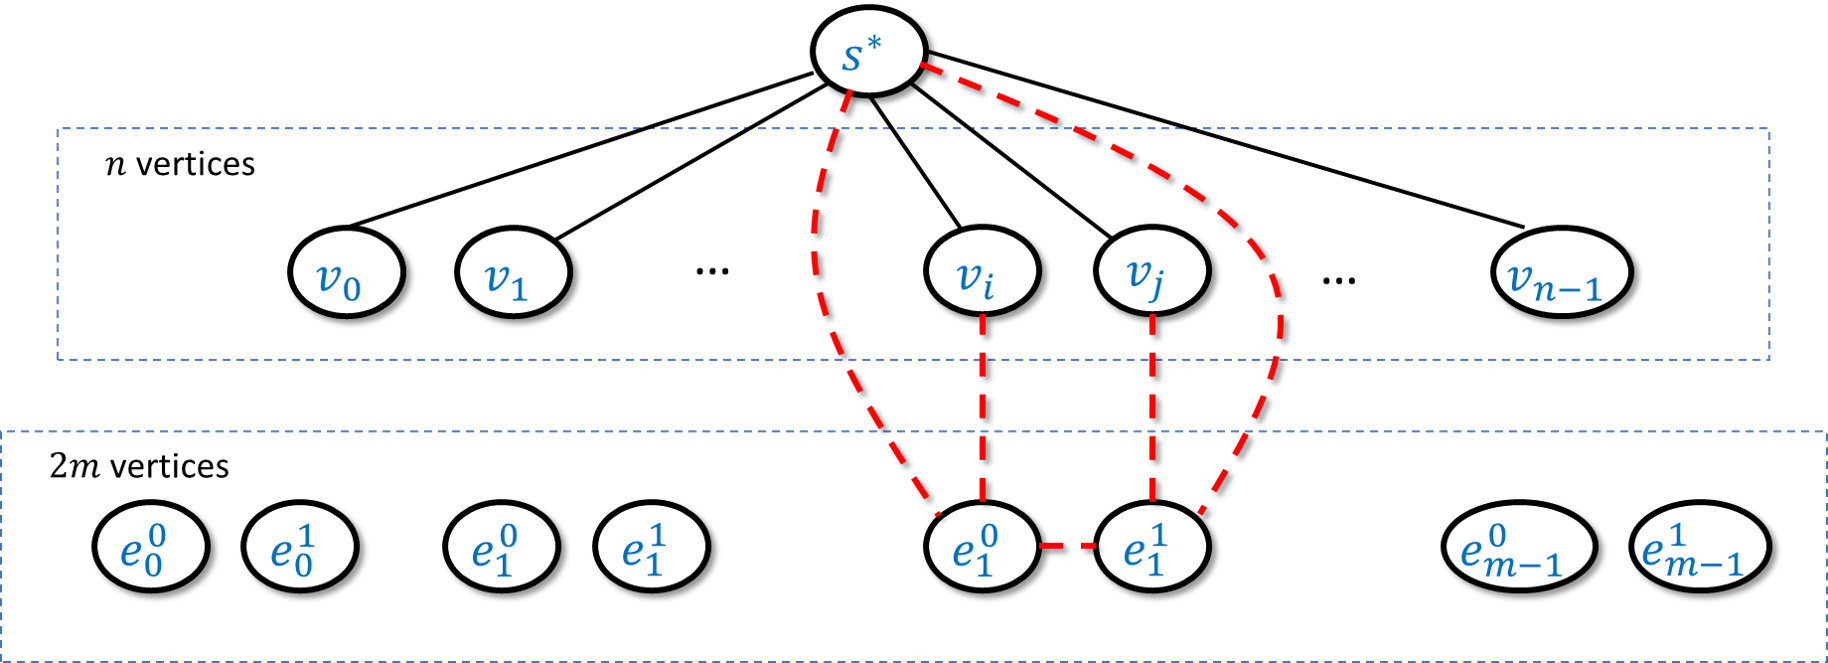
\includegraphics[width=\textwidth, height=0.25\paperheight, keepaspectratio]{../figure/iset2maxcutoverview.png}
\caption{In the reduction of \(\ensuremath{\mathit{ISET}}\) to
\(\ensuremath{\mathit{MAXCUT}}\) we map an \(n\)-vertex \(m\)-edge graph
\(G\) into the \(n+2m+1\) vertex and \(n+5m\) edge graph \(H\) as
follows. The graph \(H\) contains a special ``source'' vertex
\(s^*\),\(n\) vertices \(v_0,\ldots,v_{n-1}\), and \(2m\) vertices
\(e_0^0,e_0^1,\ldots,e_{m-1}^0,e_{m-1}^1\) with each pair corresponding
to an edge of \(G\). We put an edge between \(s^*\) and \(v_i\) for
every \(i\in [n]\), and if the \(t\)-th edge of \(G\) was \((v_i,v_j)\)
then we add the five edges
\((s^*,e_t^0),(s^*,e_t^1),(v_i,e_t^0),(v_j,e_t^1),(e_t^0,e_t^1)\). The
intent is that if cut at most one of \(v_i,v_j\) from \(s^*\) then we'll
be able to cut \(4\) out of these five edges, while if we cut both
\(v_i\) and \(v_j\) from \(s^*\) then we'll be able to cut at most three
of them.}
\label{iset2maxcutoverviewfig}
\end{figure}

\begin{proof}[Proof of \cref{isettomaxcut}] \label[proof]{We-will-transform-a-graph}

We will transform a graph \(G\) of \(n\) vertices and \(m\) edges into a
graph \(H\) of \(n+1+2m\) vertices and \(n+5m\) edges in the following
way (see also \cref{iset2maxcutoverviewfig}). The graph \(H\) contains
all vertices of \(G\) (though not the edges between them!) and in
addition \(H\) also has:\\
* A special vertex \(s^*\) that is connected to all the vertices of
\(G\)\\
* For every edge \(e=\{u,v\} \in E(G)\), two vertices \(e_0,e_1\) such
that \(e_0\) is connected to \(u\) and \(e_1\) is connected to \(v\),
and moreover we add the edges \(\{e_0,e_1 \},\{ e_0,s^* \},\{e_1,s^*\}\)
to \(H\).

\cref{isettomaxcut} will follow by showing that \(G\) contains an
independent set of size at least \(k\) if and only if \(H\) has a cut
cutting at least \(k+4m\) edges. We now prove both directions of this
equivalence:

\textbf{Part 1: Completeness.} If \(I\) is an independent \(k\)-sized
set in \(G\), then we can define \(S\) to be a cut in \(H\) of the
following form: we let \(S\) contain all the vertices of \(I\) and for
every edge \(e=\{u,v \} \in E(G)\), if \(u\in I\) and \(v\not\in I\)
then we add \(e_1\) to \(S\); if \(u\not\in I\) and \(v\in I\) then we
add \(e_0\) to \(S\); and if \(u\not\in I\) and \(v\not\in I\) then we
add both \(e_0\) and \(e_1\) to \(S\). (We don't need to worry about the
case that both \(u\) and \(v\) are in \(I\) since it is an independent
set.) We can verify that in all cases the number of edges from \(S\) to
its complement in the gadget corresponding to \(e\) will be four (see
\cref{ISETtoMAXCUTfig}). Since \(s^*\) is not in \(S\), we also have
\(k\) edges from \(s^*\) to \(I\), for a total of \(k+4m\) edges.

\textbf{Part 2: Soundness.} Suppose that \(S\) is a cut in \(H\) that
cuts at least \(C=k+4m\) edges. We can assume that \(s^*\) is not in
\(S\) (otherwise we can ``flip'' \(S\) to its complement
\(\overline{S}\), since this does not change the size of the cut). Now
let \(I\) be the set of vertices in \(S\) that correspond to the
original vertices of \(G\). If \(I\) was an independent set of size
\(k\) then would be done. This might not always be the case but we will
see that if \(I\) is not an independent set then it's also larger than
\(k\). Specifically, we define \(m_{in}=|E(I,I)|\) be the set of edges
in \(G\) that are contained in \(I\) and let \(m_{out}=m-m_{in}\) (i.e.,
if \(I\) is an independent set then \(m_{in}=0\) and \(m_{out}=m\)). By
the properties of our gadget we know that for every edge \(\{u,v\}\) of
\(G\), we can cut at most three edges when both \(u\) and \(v\) are in
\(S\), and at most four edges otherwise. Hence the number \(C\) of edges
cut by \(S\) satisfies
\(C \leq |I| + 3m_{in}+4m_{out} = |I|+ 3m_{in} + 4(m-m_{in})=|I|+4m-m_{in}\).
Since \(C = k +4m\) we get that \(|I|-m_{in} \geq k\). Now we can
transform \(I\) into an independent set \(I'\) by going over every one
of the \(m_{in}\) edges that are inside \(I\) and removing one of the
endpoints of the edge from it. The resulting set \(I'\) is an
independent set in the graph \(G\) of size \(|I|-m_{in} \geq k\) and so
this concludes the proof of the soundness condition.

\end{proof}


\begin{marginfigure}
\centering
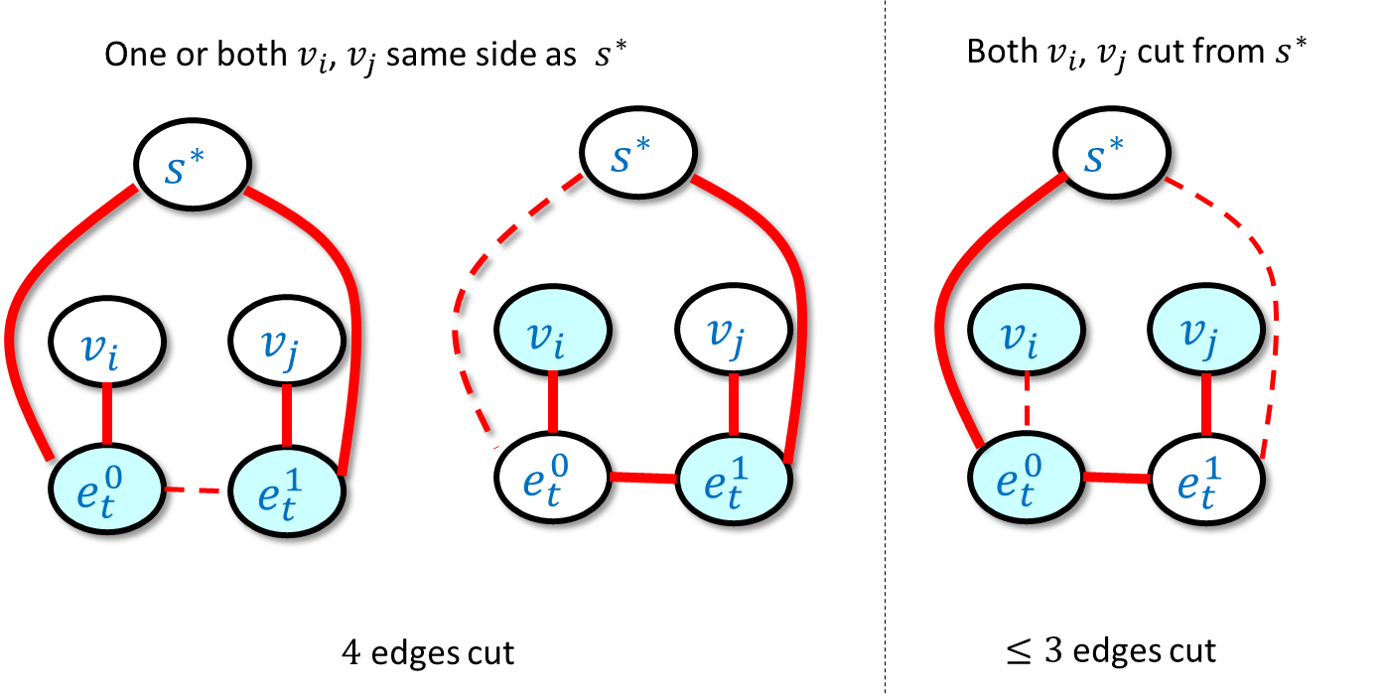
\includegraphics[width=\linewidth, height=1.5in, keepaspectratio]{../figure/iset2maxcutgadgetanalysis.png}
\caption{In the reduction of independent set to max cut, for every
\(t\in [m]\), we have a ``gadget'' corresponding to the \(t\)-th edge
\(e= \{ v_i,v_j\}\) in the original graph. If we think of the side of
the cut containing the special source vertex \(s^*\) as ``white'' and
the other side as ``blue'', then the leftmost and center figures show
that if \(v_i\) and \(v_j\) are not both blue then we can cut four edges
from the gadget. In contrast, by enumerating all possibilities one can
verify that if both \(u\) and \(v\) are blue, then no matter how we
color the intermediate vertices \(e_t^0,e_t^1\), we will cut at most
three edges from the gadget. The figure above contains only the gadget
edges and ignores the edges connecting \(s^*\) to the vertices
\(v_0,\ldots,v_{n-1}\).}
\label{ISETtoMAXCUTfig}
\end{marginfigure}


\begin{figure}
\centering
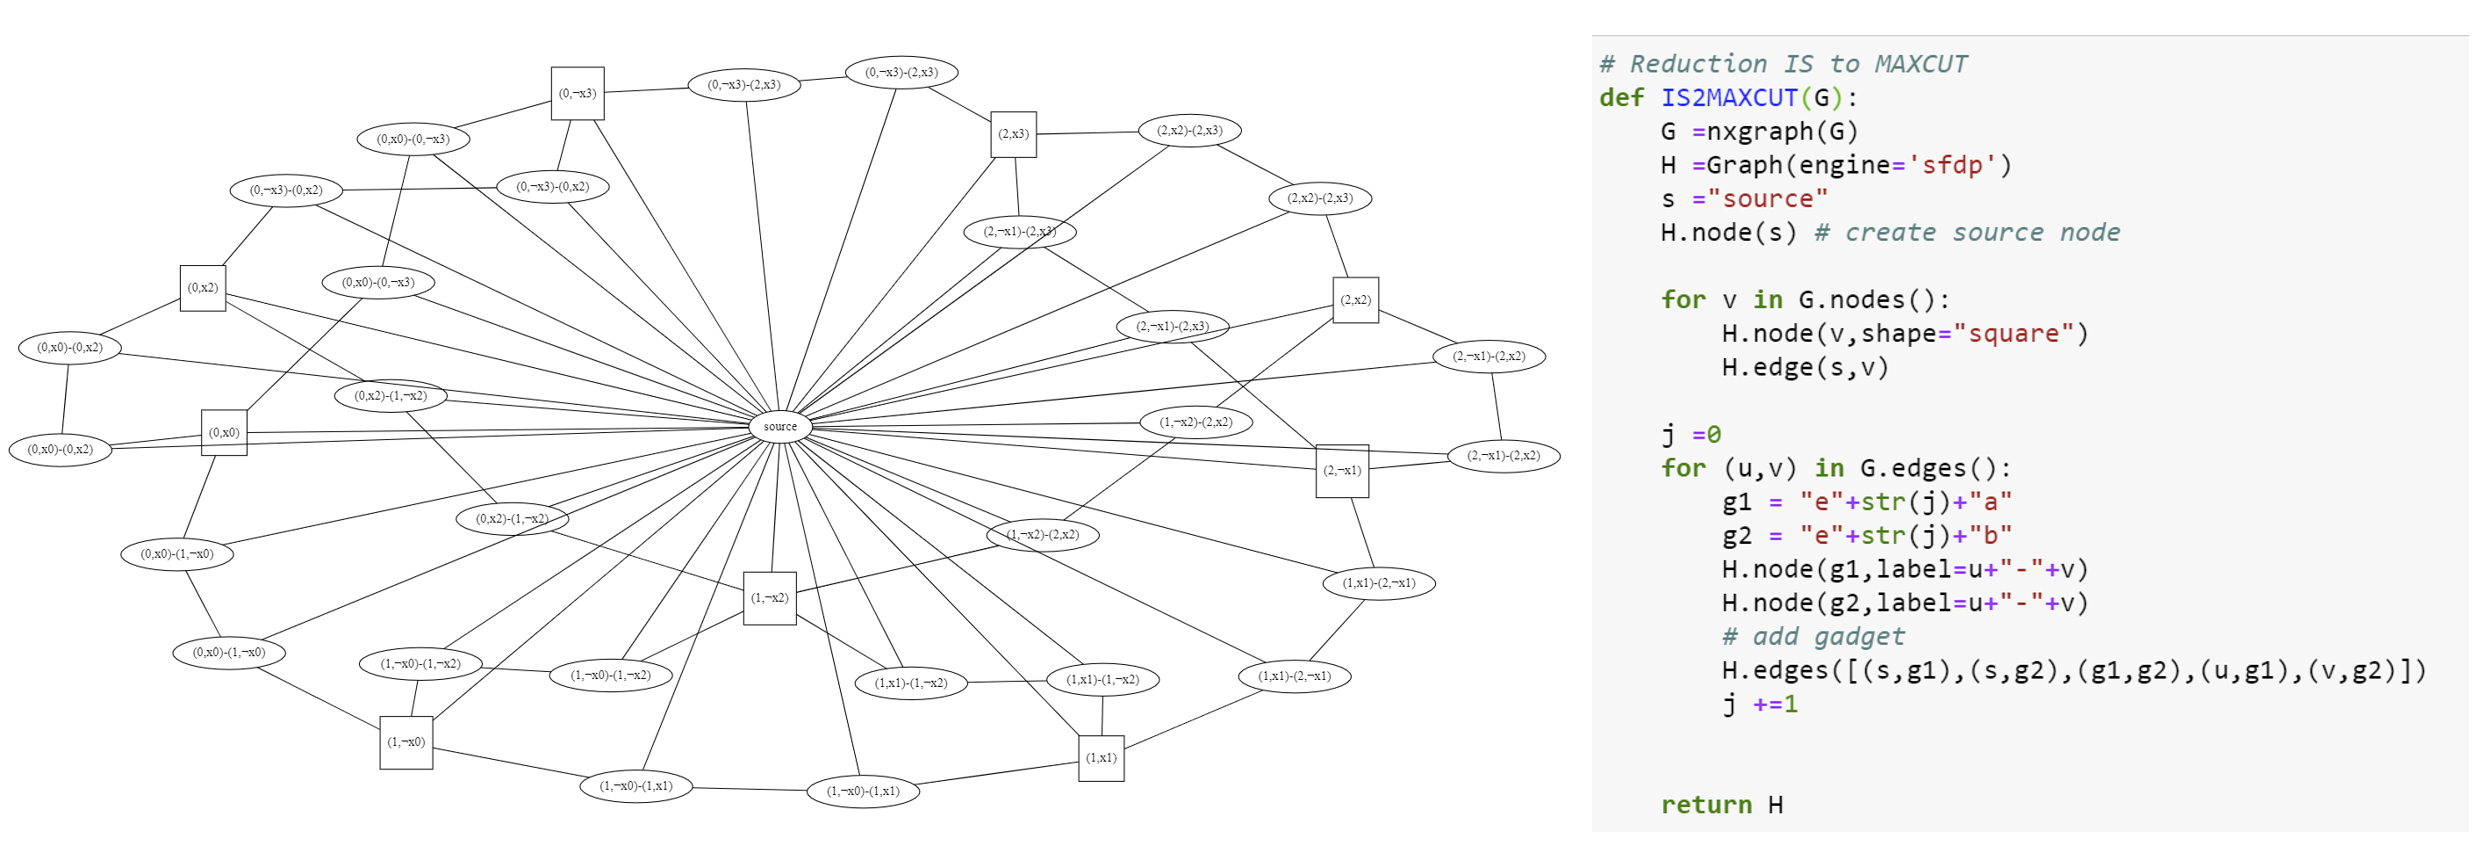
\includegraphics[width=\textwidth, height=0.25\paperheight, keepaspectratio]{../figure/is2maxcut.png}
\caption{The reduction of independent set to max cut. On the righthand
side is Python code implementing the reduction. On the lefthand side is
an example output of the reduction where we apply it to the independent
set instance that is obtained by running the reduction of \cref{isetnpc}
on the 3CNF formula
\((x_0 \vee \overline{x}_3 \vee x_2) \wedge (\overline{x}_0 \vee x_1 \vee \overline{x}_2) \wedge (\overline{x}_1 \vee x_2 \vee x_3)\).}
\label{isettomaxcutcodefig}
\end{figure}

\section{Reducing 3SAT to Longest Path}\label{Reducing-SAT-to-Longest-P}

\paragraph{Note:} This section is still a little messy; feel free to
skip it or just read it without going into the proof details. The proof
appears in Section 7.5 in Sipser's book.

One of the most basic algorithms in Computer Science is Dijkstra's
algorithm to find the \emph{shortest path} between two vertices. We now
show that in contrast, an efficient algorithm for the \emph{longest
path} problem would imply a polynomial-time algorithm for 3SAT.

\hypertarget{longpaththm}{}
\begin{theorem}[Hardness of longest path] \label[theorem]{longpaththm}

\[3\ensuremath{\mathit{SAT}} \leq_p \ensuremath{\mathit{LONGPATH}}\]

\end{theorem}


\begin{marginfigure}
\centering
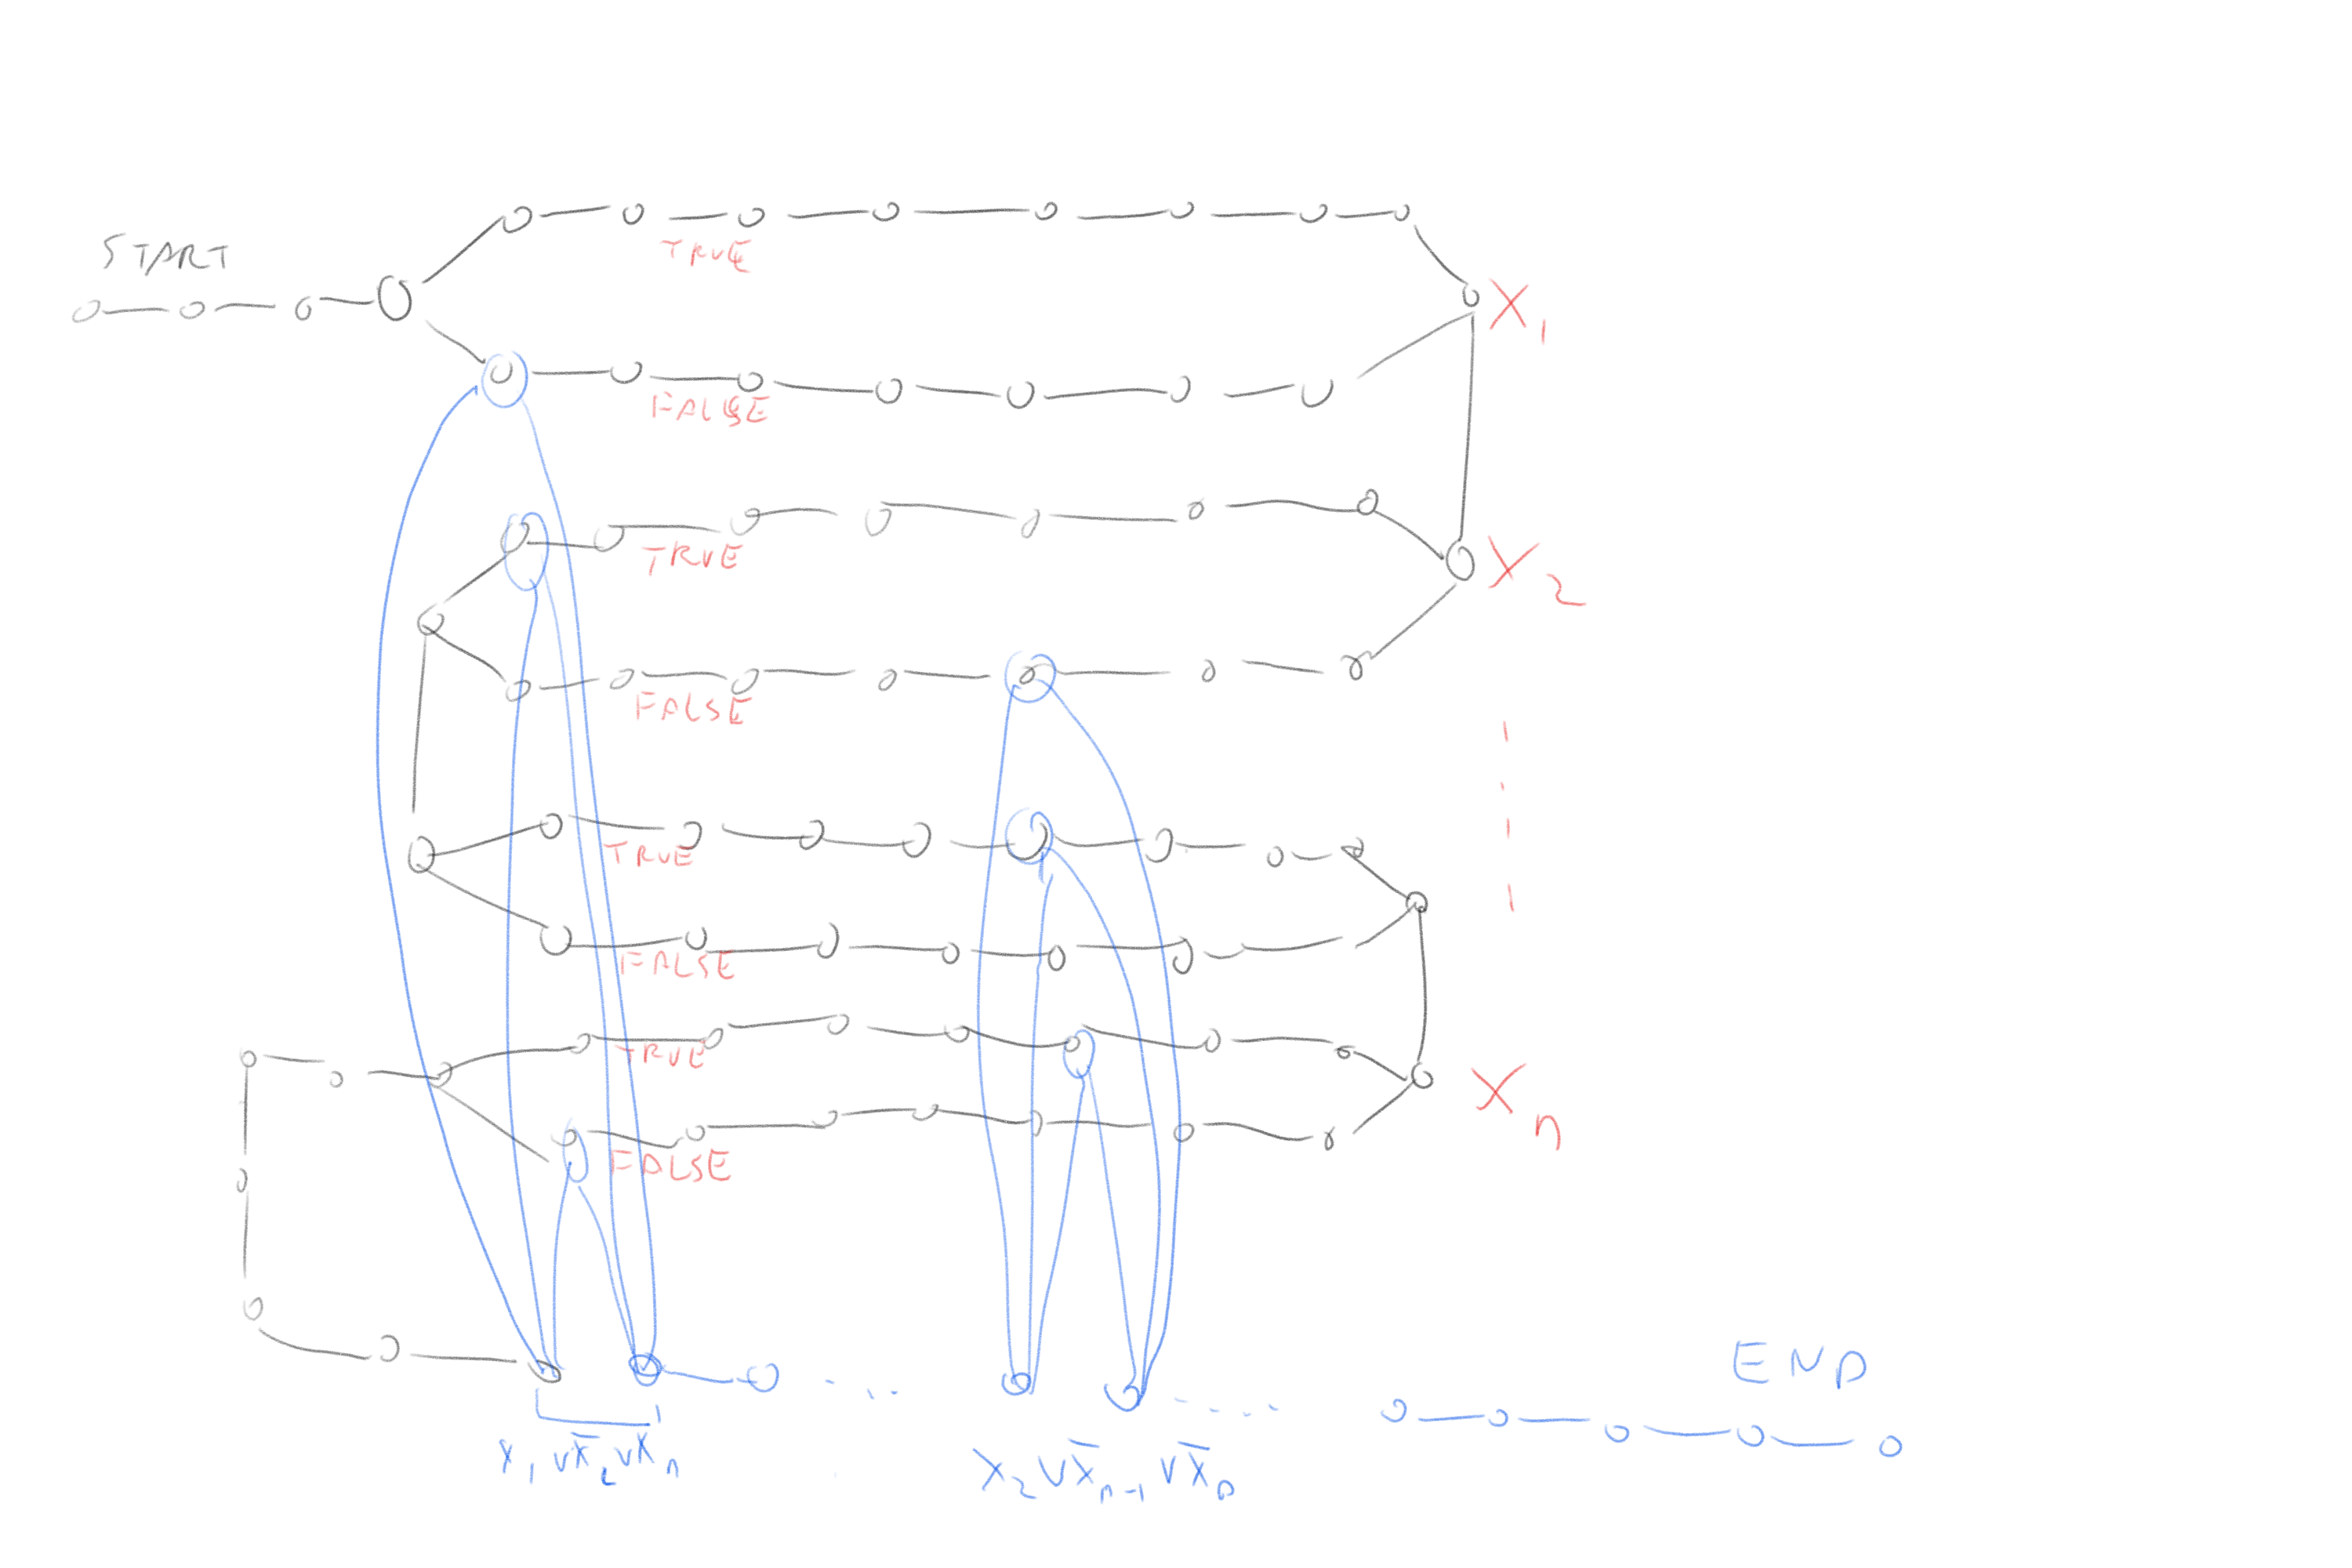
\includegraphics[width=\linewidth, height=1.5in, keepaspectratio]{../figure/3sat_longest_path_red_without_path.png}
\caption{We can transform a 3SAT formula \(\varphi\) into a graph \(G\)
such that the longest path in the graph \(G\) would correspond to a
satisfying assignment in \(\varphi\). In this graph, the black colored
part corresponds to the variables of \(\varphi\) and the blue colored
part corresponds to the vertices. A sufficiently long path would have to
first ``snake'' through the black part, for each variable choosing
either the ``upper path'' (corresponding to assigning it the value
\texttt{True}) or the ``lower path'' (corresponding to assigning it the
value \texttt{False}). Then to achieve maximum length the path would
traverse through the blue part, where to go between two vertices
corresponding to a clause such as
\(x_{17} \vee \overline{x}_{32} \vee x_{57}\), the corresponding
vertices would have to have been not traversed before.}
\label{longpathfig}
\end{marginfigure}


\begin{marginfigure}
\centering
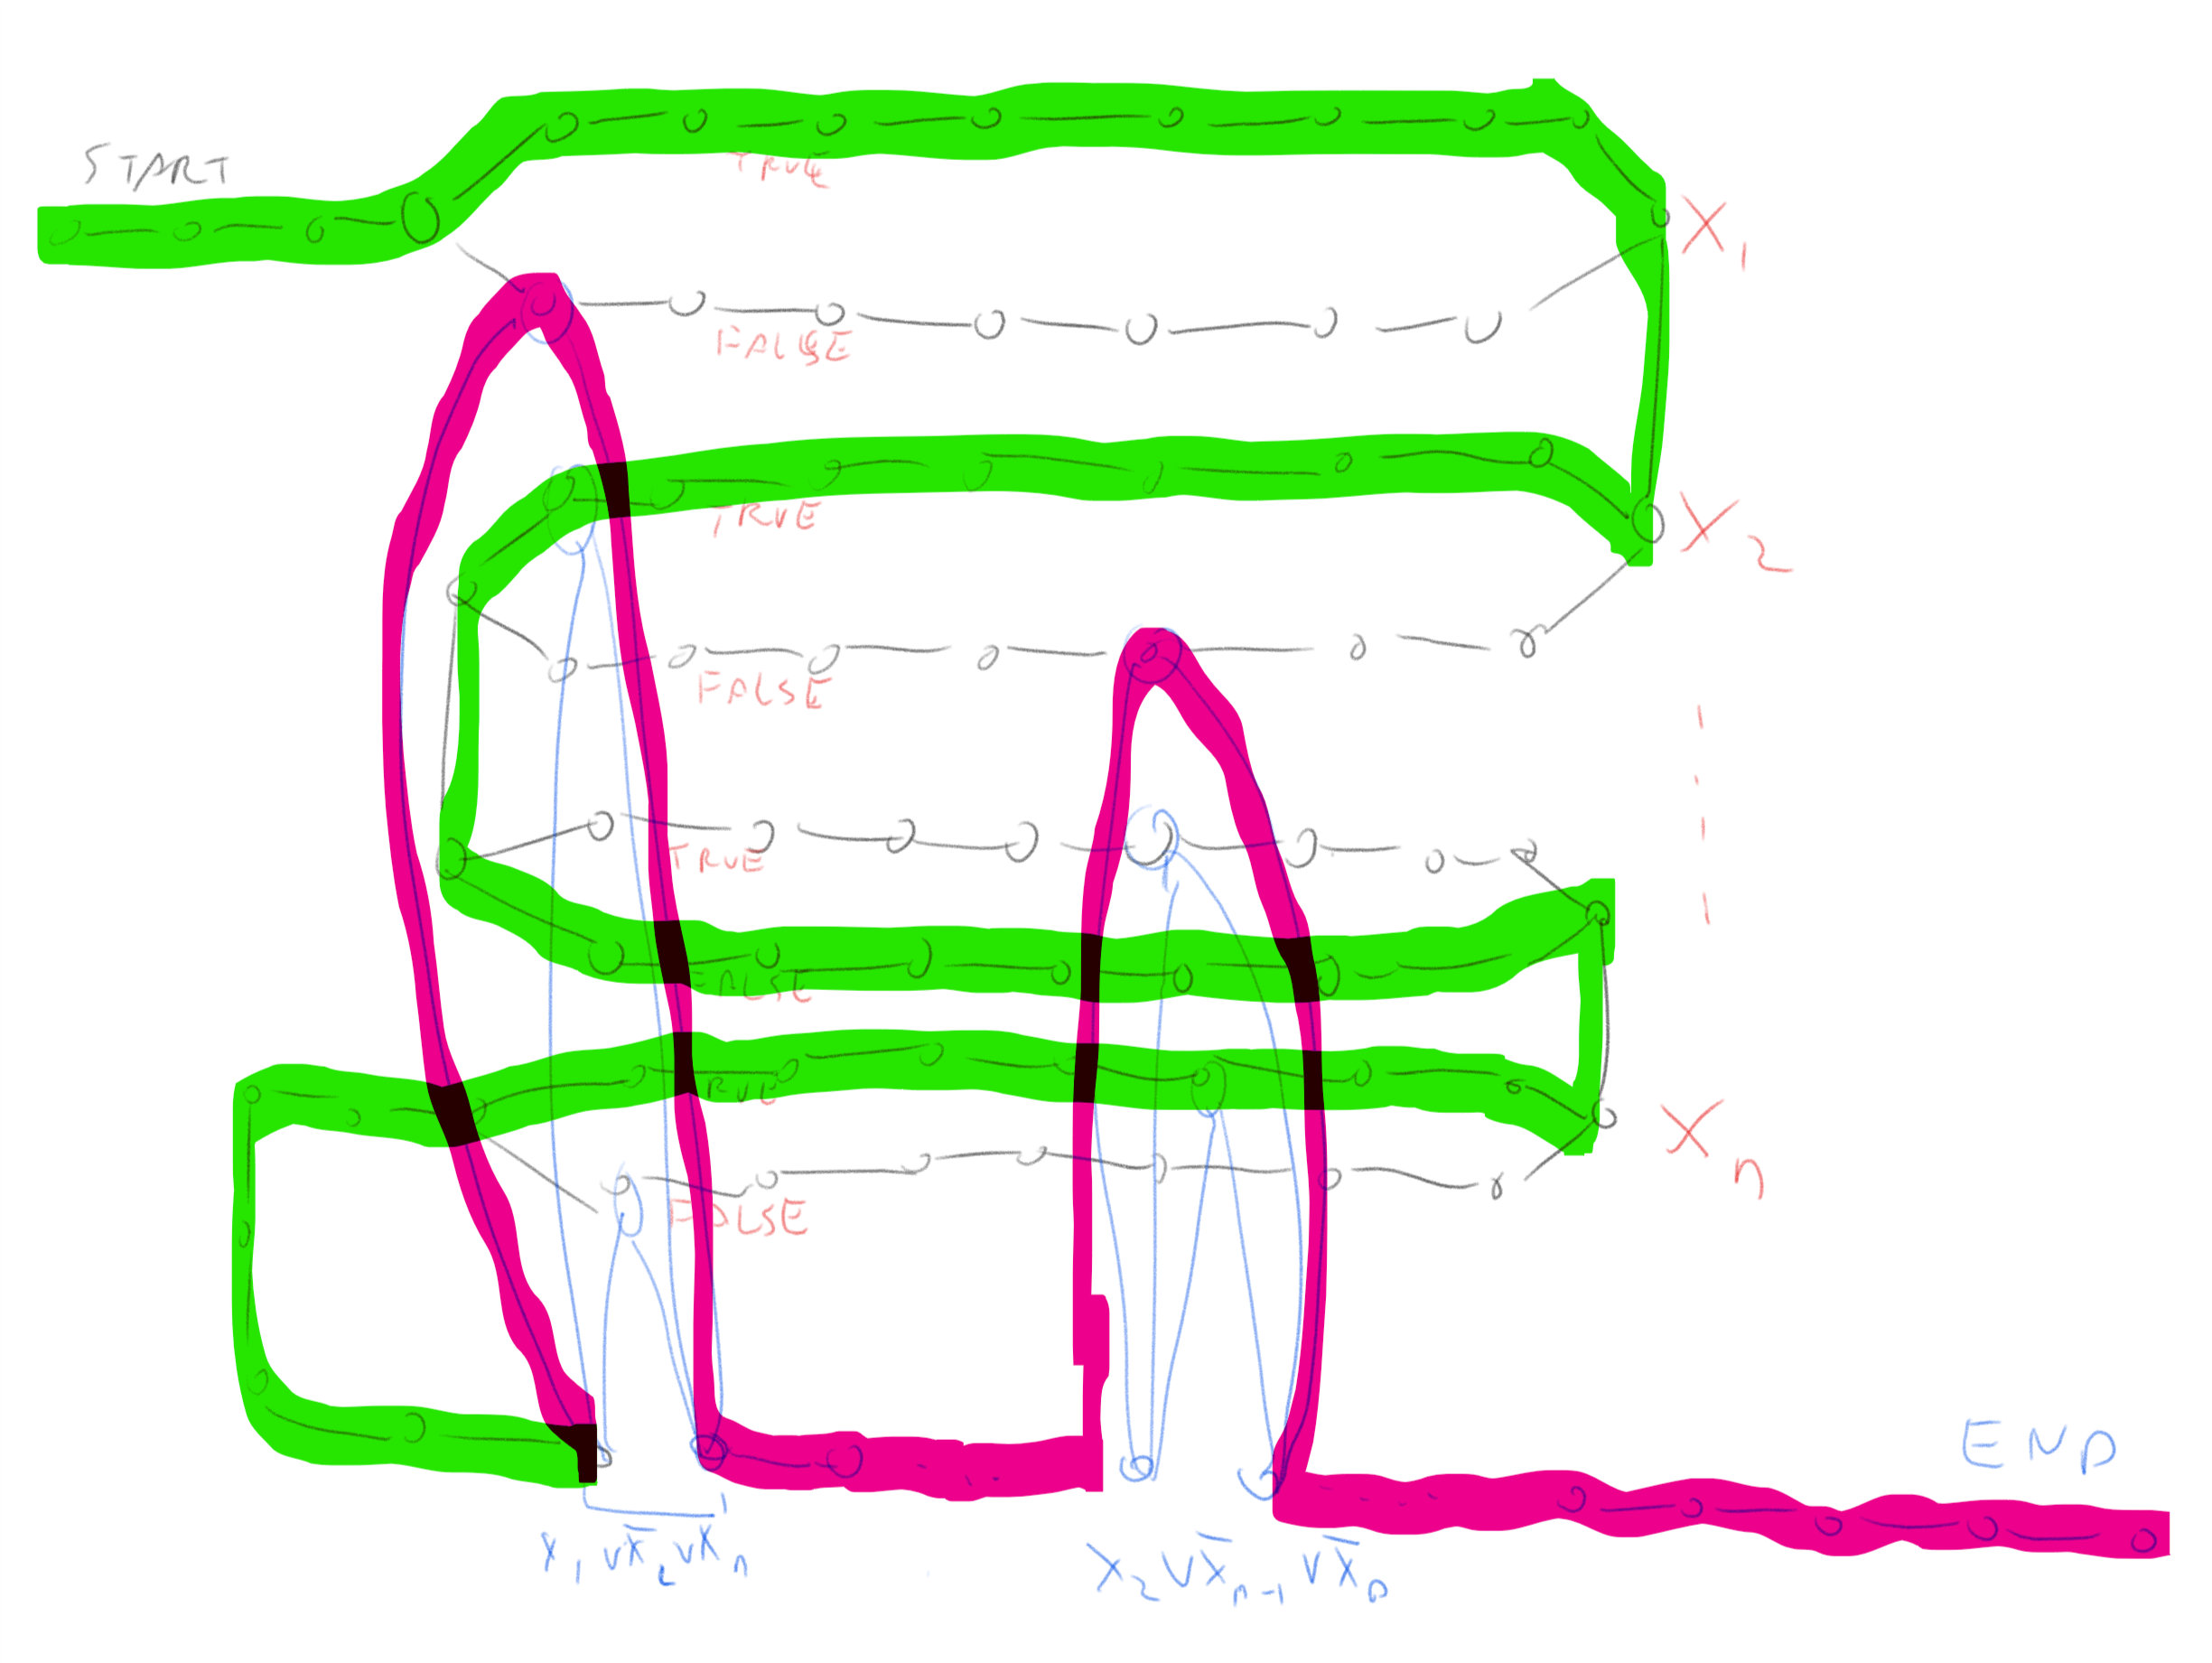
\includegraphics[width=\linewidth, height=1.5in, keepaspectratio]{../figure/3sat_to_longest_path_reduction.png}
\caption{The graph above with the longest path marked on it, the part of
the path corresponding to variables is in green and part corresponding
to the clauses is in pink.}
\label{longpathfigtwo}
\end{marginfigure}

\begin{proofidea} \label[proofidea]{To-prove-creflongpaththm-}

To prove \cref{longpaththm} need to show how to transform a 3CNF formula
\(\varphi\) into a graph \(G\) and two vertices \(s,t\) such that \(G\)
has a path of length at least \(k\) if and only if \(\varphi\) is
satisfiable. The idea of the reduction is sketched in \cref{longpathfig}
and \cref{longpathfigtwo}. We will construct a graph that contains a
potentially long ``snaking path'' that corresponds to all variables in
the formula. We will add a ``gadget'' corresponding to each clause of
\(\varphi\) in a way that we would only be able to use the gadgets if we
have a satisfying assignment.

\end{proofidea}

\begin{proof}[Proof of \cref{longpaththm}] \label[proof]{We-build-a-graph-G-that-s}

We build a graph \(G\) that ``snakes'' from \(s\) to \(t\) as follows.
After \(s\) we add a sequence of \(n\) long loops. Each loop has an
``upper path'' and a ``lower path''. A simple path cannot take both the
upper path and the lower path, and so it will need to take exactly one
of them to reach \(s\) from \(t\).

Our intention is that a path in the graph will correspond to an
assignment \(x\in \{0,1\}^n\) in the sense that taking the upper path in
the \(i^{th}\) loop corresponds to assigning \(x_i=1\) and taking the
lower path corresponds to assigning \(x_i=0\). When we are done snaking
through all the \(n\) loops corresponding to the variables to reach
\(t\) we need to pass through \(m\) ``obstacles'': for each clause \(j\)
we will have a small gadget consisting of a pair of vertices \(s_j,t_j\)
that have three paths between them. For example, if the \(j^{th}\)
clause had the form \(x_{17} \vee \overline{x}_{55} \vee x_{72}\) then
one path would go through a vertex in the lower loop corresponding to
\(x_{17}\), one path would go through a vertex in the upper loop
corresponding to \(x_{55}\) and the third would go through the lower
loop corresponding to \(x_{72}\). We see that if we went in the first
stage according to a satisfying assignment then we will be able to find
a free vertex to travel from \(s_j\) to \(t_j\). We link \(t_1\) to
\(s_2\), \(t_2\) to \(s_3\), etc and link \(t_m\) to \(t\). Thus a
satisfying assignment would correspond to a path from \(s\) to \(t\)
that goes through one path in each loop corresponding to the variables,
and one path in each loop corresponding to the clauses. We can make the
loop corresponding to the variables long enough so that we must take the
entire path in each loop in order to have a fighting chance of getting a
path as long as the one corresponds to a satisfying assignment. But if
we do that, then the only way if we are able to reach \(t\) is if the
paths we took corresponded to a satisfying assignment, since otherwise
we will have one clause \(j\) where we cannot reach \(t_j\) from \(s_j\)
without using a vertex we already used before.

\end{proof}

\subsection{Summary of relations}\label{Summary-of-relations}

We have shown that there are a number of functions \(F\) for which we
can prove a statement of the form ``If \(F\in \mathbf{P}\) then
\(3\ensuremath{\mathit{SAT}} \in \mathbf{P}\)''. Hence coming up with a
polynomial-time algorithm for even one of these problems will entail a
polynomial-time algorithm for \(3\ensuremath{\mathit{SAT}}\) (see for
example \cref{reductiondiagramfig}). In \cref{cooklevinchap} we will
show the inverse direction (``If
\(3\ensuremath{\mathit{SAT}} \in \mathbf{P}\) then
\(F\in \mathbf{P}\)'') for these functions, hence allowing us to
conclude that they have \emph{equivalent complexity} to
\(3\ensuremath{\mathit{SAT}}\).


\begin{figure}
\centering
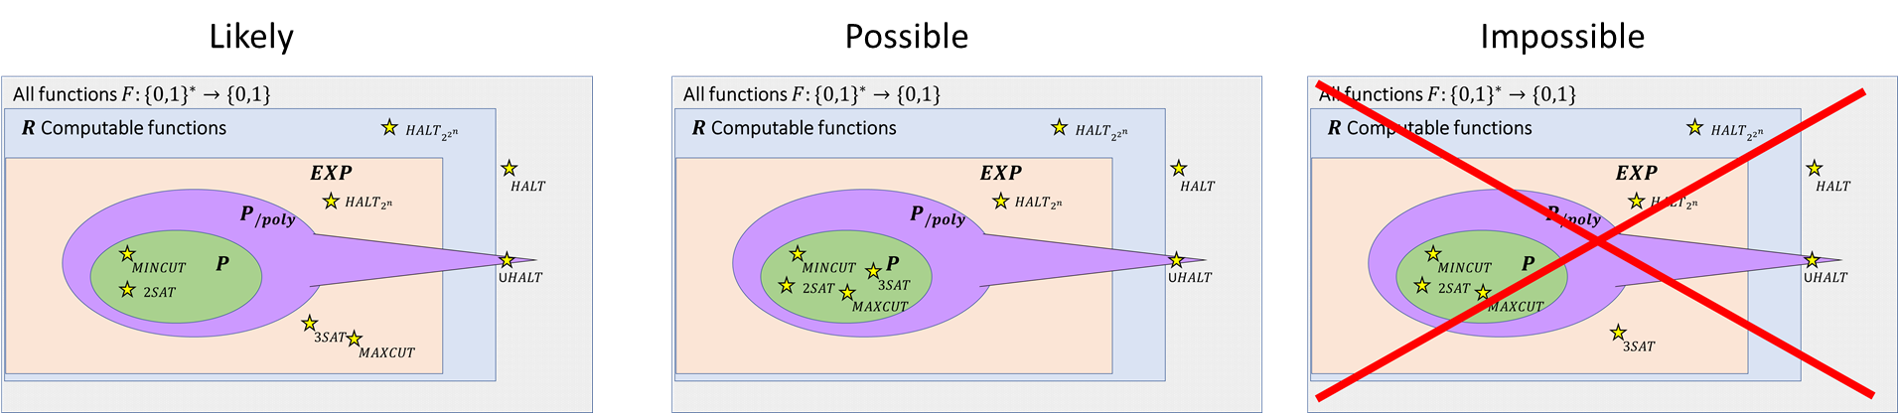
\includegraphics[width=\textwidth, height=0.25\paperheight, keepaspectratio]{../figure/reduction_inc_diagram.png}
\caption{So far we have shown that \(\mathbf{P} \subseteq \mathbf{EXP}\)
and that several problems we care about such as
\(3\ensuremath{\mathit{SAT}}\) and \(\ensuremath{\mathit{MAXCUT}}\) are
in \(\mathbf{EXP}\) but it is not known whether or not they are in
\(\mathbf{EXP}\). However, since
\(3\ensuremath{\mathit{SAT}} \leq_p \ensuremath{\mathit{MAXCUT}}\) we
can rule out the possiblity that
\(\ensuremath{\mathit{MAXCUT}} \in \mathbf{P}\) but
\(3\ensuremath{\mathit{SAT}} \not\in \mathbf{P}\). The relation of
\(\mathbf{P_{/poly}}\) to the class \(\mathbf{EXP}\) is not known. We
know that \(\mathbf{EXP}\) does not contain \(\mathbf{P_{/poly}}\) since
the latter even contains uncomputable functions, but we do not know
whether ot not \(\mathbf{EXP} \subseteq \mathbf{P_{/poly}}\) (though it
is believed that this is not the case and in particular that both
\(3\ensuremath{\mathit{SAT}}\) and \(\ensuremath{\mathit{MAXCUT}}\) are
not in \(\mathbf{P_{/poly}}\)).}
\label{reductiondiagramfig}
\end{figure}

\begin{recap} \label[recap]{The-computational-complex}

\begin{itemize}
\item
  The computational complexity of many seemingly unrelated computational
  problems can be related to one another through the use of
  \emph{reductions}.
\item
  If \(F \leq_p G\) then a polynomial-time algorithm for \(G\) can be
  transformed into a polynomial-time algorithm for \(F\).
\item
  Equivalently, if \(F \leq_p G\) and \(F\) does \emph{not} have a
  polynomial-time algorithm then neither does \(G\).
\item
  We've developed many techniques to show that
  \(3\ensuremath{\mathit{SAT}} \leq_p F\) for interesting functions
  \(F\). Sometimes we can do so by using \emph{transitivity} of
  reductions: if \(3\ensuremath{\mathit{SAT}} \leq_p G\) and
  \(G \leq_p F\) then \(3\ensuremath{\mathit{SAT}} \leq_p F\).
\end{itemize}

\end{recap}

\section{Exercises}\label{Exercises}

\section{Bibliographical notes}\label{reductionsbibnotes}

Several notions of reductions are defined in the literature. The notion
defined in \cref{reduction-def} is often known as a \emph{mapping
reduction}, \emph{many to one reduction} or a \emph{Karp reduction}.

The \emph{maximal} (as opposed to \emph{maximum}) independent set is the
task of finding a ``local maximum'' of an independent set: an
independent set \(S\) such that one cannot add a vertex to it without
losing the independence property (such a set is known as a \emph{vertex
cover}). Unlike finding a \emph{maximum} independent set, finding a
\emph{maximal} independent set can be done efficiently by a greedy
algorithm, but this local maximum can be much smaller than the global
maximum.

Reduction of independent set to max cut taken from
\href{https://people.engr.ncsu.edu/mfms/Teaching/CSC505/wrap/Lectures/week14.pdf}{these
notes}. Image of Hamiltonian Path through Dodecahedron by
\href{https://commons.wikimedia.org/wiki/File:Hamiltonian_path.svg}{Christoph
Sommer}.

We have mentioned that the line between reductions used for algorithm
design and showing hardness is sometimes blurry. An excellent example
for this is the area of \emph{SAT Solvers} (see
\cite{gomes2008satisfiability}). In this field people use algorithms for
SAT (that take exponential time in the worst case but often are much
faster on many instances in practice) together with reductions of the
form \(F \leq_p \ensuremath{\mathit{SAT}}\) to derive algorithms for
other functions \(F\) of interest.
